\documentclass[11pt]{article}
\usepackage{doi}

% -----------------------------
% Packages
% -----------------------------
\usepackage[margin=1in]{geometry}
\usepackage{setspace}
\usepackage{amsmath,amssymb,amsfonts,amsthm}
\usepackage{mathtools}
\usepackage{bm}
\usepackage{graphicx}
\graphicspath{
  {figures/}
}
\usepackage{xcolor}
\usepackage{booktabs}
\usepackage{float}
\usepackage{placeins}
\usepackage{hyperref}
\usepackage[numbers,sort&compress]{natbib}
\usepackage{tikz}
\usetikzlibrary{arrows.meta}
\usepackage{microtype}
\usepackage{natbib}
% -----------------------------
% Formatting
% -----------------------------
\setstretch{1.08}
\setlength{\parskip}{0.35em}
\setlength{\parindent}{0pt}

% Set this switch to \originalintroductiontrue to compile the previous
% introduction retained below for comparison.
\newif\iforiginalintroduction
\originalintroductionfalse

% -----------------------------
% Macros
% -----------------------------
\newcommand{\E}{\mathbb{E}}
\newcommand{\Prob}{\mathbb{P}}
\newcommand{\R}{\mathbb{R}}
\newcommand{\dd}{\,\mathrm{d}}

\newcommand{\Qpres}{Q}
\newcommand{\Ppos}{P}
\newcommand{\Nneg}{N}
\newcommand{\Fimm}{F}

% -----------------------------
% Title block
% -----------------------------
\title{\textbf{A mechanistic modeling framework for CD8$^{+}$ T-cell antigen immunogenicity}}
\author{Marcus Thomas$^{1}$ \quad Marta Luksza$^{1}$}
\date{}

\begin{document}
\maketitle

\begin{flushleft}
\small
$^{1}$\textit{Memorial Sloan Kettering Cancer Center, New York, NY, USA}\\
\end{flushleft}

% ============================================================
% ABSTRACT
% ============================================================
\begin{abstract}
CD8$^{+}$ T-cell immunogenicity depends on antigen presentation, the
availability of cognate T-cell receptors after selection, and productive
peptide--MHC--TCR interaction. We develop a mechanistic score that represents
these requirements through the multiplicative response
$F=P\cdot N\cdot Q\cdot\Pi$. Recognition geometry, selection decisions, and
alternative constructions of the modeled HLA environment define candidate
minimal-epitope scores. Long-peptide assays additionally require an aggregation
rule over candidate epitope--HLA presentations. These choices jointly specify
the composite models confronted with four refutation datasets: resolved NCI
neoepitope observations, PDAC vaccine responses, and SARS-CoV-2 spike-mutation
and non-spike responses. A directed supported-superiority tournament asks
which models remain admissible in every context under declared prevalence,
case-mix, and computational challenges. The full comparison exposes each
complete model to all four datasets, but requires extensive score construction
and pairwise assessment. We formulate sequential approximations that expand
NCI-retained regimes into long-peptide models and distinguish restrictions on
eligible candidates from restrictions on their challengers. The resulting
design preserves unresolved alternatives and makes explicit which criticisms
a tractable comparison can omit.
\end{abstract}

% ============================================================
% INTRODUCTION
% ============================================================
\iforiginalintroduction
% ----------------------------------------------------------------
% ORIGINAL INTRODUCTION (retained for comparison)
% ----------------------------------------------------------------
Immunogenicity is not an intrinsic property of an antigen alone. Whether a peptide elicits a CD8+ T-cell response depends on a chain of host-contextual events, including peptide processing, presentation by MHC molecules, the availability of compatible T-cell receptors, and productive receptor engagement. This creates a natural limit for purely statistical predictors trained on sparse immunogenicity labels: they may learn cohort-specific correlates of response without learning an approximately correct mechanism for why a peptide should be recognized.  Further, the data requirements for moving beyond the sparse regime are truly enormous (and impractical) given the diversity of biologically possible peptides, TCR sequences and MHC alleles.  
Failures of generalization (e.g. to new datasets or biological contexts) reflect failure to adequately model the data-generating process.
We therefore take the direct approach of modeling the data generating process (causation) rather than the statistics of the data (correlation). We treat downstream evaluation on datasets as opportunities for refutation rather than validation. 


CD8$^{+}$ T-cell immunogenicity is a causal phenomenon.
A T-cell response arises only when several necessary conditions jointly
obtain.
The antigen must be processed into a short linear peptide and
presented on at least one of the host's MHC class~I molecules, forming
the peptide--MHC (pMHC) complex that defines the target of recognition.
Conditional on presentation, a response further requires the existence
of TCRs that bind the complex with sufficient stability and affinity to
trigger activation.
And conditional on the existence of such receptors, a response requires
that they be present in the mature repertoire: T-cells must have
survived thymic selection, a developmental process that filters the
pre-selection repertoire through interactions with self
peptide--MHC complexes.

Thymic selection imposes two sequential filters.
Positive selection eliminates T-cells whose receptors are
insufficiently self-reactive; those that fail to engage self-peptides
with moderate affinity die by neglect.
Negative selection eliminates T-cells with excessive self-reactivity;
those that bind self-peptides too strongly are deleted.
The combined effect defines a recognition window: T-cells must
accumulate enough moderate self-interactions to pass positive selection
but not so many strong interactions that they trigger deletion.
Quantitative considerations indicate that thymic deletion cannot act
as a complete or exhaustive screening
process~\citep{MoraWalczak2023}.
It is therefore more accurate to treat negative selection pressure as an aggregate filter capturing the combined action of central and peripheral tolerance mechanisms, rather than as a model of thymic deletion alone.
The self-peptidome, together with the host's HLA profile, determines
which T-cells survive these filters and therefore constrains which
foreign epitopes can be recognized.

Standard supervised learning approaches commonly associate some sequence or structural information 
with immunogenicity labels. Here the relevant causal unit is broader:
immunogenicity depends on the peptide, the host's HLA and self-peptide context,
and antigen exposure. The same peptide can therefore elicit different responses
across hosts or exposure levels. Pooling individuals combines distinct
data-generating processes, and apparent label variability carries biological
structure from unmeasured context and concentration. At low abundance a peptide
may remain below activation thresholds; at higher abundance it may cross them.
Prospective prediction consequently requires models that represent these
contextual sources of variation.

TCR-agnostic prediction is nonetheless principled.
Individuals with the same HLA background present similar
self-peptide repertoires during thymic development and therefore impose
similar selection constraints, even though their post-selection TCR
repertoires share essentially no sequences.
Thymic selection funnels the diversity of VDJ recombination outputs
through a structured filter defined by self-recognition patterns.
The resulting post-selection repertoire inherits lower-dimensional
structure from the self-peptidome rather than from TCR sequence
identity.
A formal argument, developed in the Supplementary Information
Section, shows that repertoire-level
recognition can be expressed as a functional of the self-peptide
landscape and a profile-level cross-reactivity kernel, without
enumerating TCR sequences.
This supports reasoning about immunogenicity at the level of
epitopes, distances, and presentation weights.

We introduce a mechanistic--learning framework built on these
observations.
The model combines competitive peptide presentation, selection-conditioned
TCR availability, and HLA-conditioned evidence of productive recognition. We
use resolved neoepitope data to eliminate unsupported transferable parameter
regimes and then evaluate the resulting scores in three external
peptide-response cohorts.
We then compare every composite model with every other composite model in
both directions. A proposed replacement is retained only when its advantage
meets the declared requirements in all three external settings.

We use \emph{generalization} to mean the applicability of a conjectured
regularity, mechanism, or model relation beyond the particular observations
and biological circumstances that informed it. The object of a generalization
claim may be a mechanistic relation, a component construction, a transferable
parameter regime, an aggregation rule, or a composite model.
Generalization is therefore claim- and context-relative and spans these levels.
We evaluate it through explicitly named biological context shifts. Estimating
expected performance under repeated train--test sampling is a separate
inferential task.

We organize the empirical evidence as \emph{refutation datasets}. A refutation
dataset is defined here by its evidential role: it brings specified
observations to bear on a conjecture and can eliminate a candidate when the
declared criteria fail. Refutation can operate during construction and again
when external evidence confronts a transfer claim in a new biological context.
Evidence that eliminates some
candidates also becomes construction evidence for the candidates that survive.
The retained construction choices are frozen before they are incorporated into
composite models and carried into subsequent datasets, which provide further
opportunities for failure.

The NCI tumor-infiltrating-lymphocyte neoepitope cohort provides the
construction-stage refutation data. Its observations resolve both the minimal
epitope and its restricting HLA allele. Three biologically distinct
long-peptide datasets supply this external evidence. The PDAC cohort consists
of personalized tumor-vaccine neoantigens. The other two are SARS-CoV-2 cohorts
distinguished by antigen source and immune history: the spike-mutation cohort
measures responses to spike-mutation peptides in vaccinated healthy donors,
whereas the non-spike cohort measures responses to non-spike peptides in
unvaccinated convalescent patients. These settings vary disease, antigen source,
and immune history. We preserve them as named, context-specific opportunities
to refute transfer claims: a proposed replacement must survive each external
setting separately.

The external comparison concerns composite models with two levels.
At the first level, the mechanistic model assigns a score to a candidate
minimal epitope paired with a restricting HLA allele. We call this resolved-pair
scoring Level~1 (\(\mathrm{L1}\)). The external PDAC and SARS-CoV-2 labels,
however, belong to long peptides that can contain several candidate minimal
epitopes and can be presented by several HLA alleles. A second operation must
therefore combine the candidate \(\mathrm{L1}\) scores into one score for the
labeled long-peptide experimental unit. We call this long-peptide aggregation
Level~2 (\(\mathrm{L2}\)).

This experimental resolution lets the NCI cohort inform the first level. For
every candidate recognition geometry and selection-decision regime, exposure
is maximized within each observation by a common label-blind rule. The NCI
labels then eliminate most of those regimes, leaving one metric-specific
non-exposure regime for each construction of the mechanistic score. Since an
NCI observation already resolves the epitope--HLA pair, it supplies no
long-peptide aggregation problem with which to compare the Level~2 rules.
Those rules enter when the frozen NCI regimes are carried into the three
external long-peptide contexts. Pairing an NCI-retained component construction
with an L2 rule defines a composite model: the conjecture under comparison. Its
output is one score for each labeled long-peptide unit in every external cohort.

Those outputs provide paired evidence for an eliminative question: should
composite model A replace composite model B across the represented biological
contexts? The claim A over B asks whether A's advantage warrants replacing B
with A; B over A asks the reverse. A direction is retained only when it meets
the declared superiority requirements in PDAC and both SARS-CoV-2 cohorts.
Applying both questions to every pair yields the complete directed round robin.
The retained claims form a graph, with an arrow from A to B recording evidence
for replacing B with A.

This procedure can retain several composite models rather than select a single winner.
After models linked by cycles of supported replacement claims are treated as a
group, a model is non-dominated when no arrow enters that group from another.
We call this non-dominated set ``corroborated'' under the declared
context-specific refutation criteria. This records survival of the represented
replacement opportunities; relations among survivors and claims beyond those
contexts remain open. PDAC also motivates revising the composite models. We
will compare the original full-cohort survivor set with a context-revised
analysis that removes
splenectomy-positive patients and adds the vaccine-conditioned score. This
continues conjecture and criticism using PDAC evidence.

\else
% ----------------------------------------------------------------
% RECONCEIVED INTRODUCTION (active by default)
% ----------------------------------------------------------------
Candidate antigens vastly outnumber those that can be tested experimentally.
Predictive models are therefore used to prioritize peptides for immune
monitoring, vaccine design, and therapeutic development. Predictive models are
constructed from observations obtained in particular hosts, diseases, exposure
conditions, and assays. The models are then used to prioritize candidate
antigens under different combinations of those circumstances.

Many approaches address this problem by associating observed immunogenicity
labels with molecular descriptions of the interacting participants. These
descriptions may include peptide sequence and structure, MHC sequence and
structure, and, when available, TCR sequence or structural information.
Increasing the richness of this representation can better characterize
molecular compatibility. It does not, however, specify whether the represented
interaction is realized within the biological circumstances required to
produce a response.

CD8$^{+}$ T-cell immunogenicity is not an intrinsic property of either an
antigen or a peptide--MHC--TCR configuration described by sequence and
structure alone; molecular compatibility is therefore insufficient to
characterize it. Sequence and structure constrain which molecular interactions
are possible, but they do not determine whether the biological process
producing a response occurs. The antigen must be processed into a short linear
peptide and presented at sufficient abundance on at least one of the host's MHC
class~I molecules. Cognate TCRs must be present in the mature repertoire, and
the resulting peptide--MHC--TCR interaction must occur under conditions that
permit activation. We therefore treat immunogenicity as a context-dependent
tendency for this biological process to produce a response, rather than as a
fixed attribute of the molecular participants considered in isolation.

This context dependence changes how immunogenicity labels should be
interpreted. When antigen supply,
competitive presentation, repertoire selection, immune history, or exposure
are absent from the modeled object, the same represented molecular
configuration can correspond to different biological situations and different
outcomes. Pooling observations while suppressing these distinctions collapses
biologically different response-generating circumstances into the same modeled
input. The resulting label variability is not necessarily unstructured noise.
A peptide may remain below an activation threshold in one setting and cross it
in another; a structurally compatible receptor may exist before selection but
be absent from the mature repertoire; and the same peptide may occupy very
different shares of presentation capacity in different HLA and peptide
environments.

We therefore conjecture a mechanistic decomposition of the response-generating
process. The model combines competitive peptide presentation,
selection-conditioned TCR availability, and HLA-conditioned evidence of
productive recognition. The decomposition does not establish that these
components are complete or true. It makes explicit claims about how response
is produced and separates choices that can be criticized at different levels.

We use \emph{generalization} to mean the applicability of a conjectured
regularity, mechanism, or model relation beyond the observations and biological
circumstances that informed its construction. The object of a generalization
claim may be a mechanistic relation, a component construction, a transferable
parameter regime, an aggregation rule, or a composite model. Generalization is
therefore claim- and context-relative and spans these levels. It is examined
here through explicitly named changes in biological context. Estimating
expected performance under repeated train--test sampling from a presumed
population law is a separate inferential task.

We organize the empirical evidence as \emph{refutation datasets}. A refutation
dataset brings specified observations to bear on a conjecture and can eliminate
a candidate when the declared criteria fail. The NCI
tumor-infiltrating-lymphocyte neoepitope cohort resolves minimal epitopes and
restricting HLA alleles. The PDAC cohort measures responses to personalized
tumor-vaccine neoantigens. Two SARS-CoV-2 cohorts differ in antigen source and
immune history: the spike-mutation cohort measures responses in vaccinated
healthy donors, whereas the non-spike cohort measures responses in unvaccinated
convalescent patients. These settings supply distinct opportunities for
criticism without being treated as draws from a common population.

Their experimental resolution determines which model implications can be
examined. Level~1 (\(\mathrm{L1}\)) assigns a score to a minimal epitope paired
with a restricting HLA allele. NCI observations are scored at this level. The
PDAC and SARS-CoV-2 labels belong to long peptides containing several candidate
minimal epitopes that may be presented by several HLA alleles. Level~2
(\(\mathrm{L2}\)) therefore combines their candidate \(\mathrm{L1}\) scores into
one score for the labeled long-peptide experimental unit.

Recognition geometry, a selection-decision regime, a component construction,
and an \(\mathrm{L2}\) rule together specify a composite model. NCI can
criticize its resolved-pair predictions but cannot distinguish models that
differ only in \(\mathrm{L2}\). The long-peptide contexts can distinguish those
models and can also expose deficiencies in their underlying \(\mathrm{L1}\)
scores. This complementary resolution motivates comparing complete composite
models across all four datasets. Supported pairwise losses determine which
models remain admissible in every context; the evidence need not identify a
single survivor. Computational restrictions may require a sequential
comparison, whose scope depends on which candidates and challengers it retains.

\fi




% ============================================================
% MECHANISTIC MODEL
% ============================================================

\section{A mechanistic model of immunogenicity}
CD8$^{+}$ T-cell response to an antigen requires that the antigen is presented on class I MHC molecules, that there are available cognate TCRs, and that pMHC-TCR binding is sufficiently stable for the necessary downstream processes to complete. We define immunogenicity as the tendency for an antigen, specifically a minimal class I epitope $e$ in an appropriate context, to elicit such a response.

We quantify the post-immunological selection immunogenicity of an epitope--HLA pair $(e,h)$ as
\begin{equation}
F(e,h,\mathcal{H},\mathcal{S};\theta)
= P(e,\mathcal{H},\mathcal{S};\theta)\;\cdot\;N(e,\mathcal{H},\mathcal{S};\theta)\;\cdot\;Q(e,h,\mathcal{H},\mathcal{S})
\;\cdot\;\Pi(e,h),
\label{eq:F_full}
\end{equation}
where $Q$ quantifies pMHC abundance;
$P \cdot N$ represents the availability of cognate TCRs capable of recognizing $(e,h)$ following positive and negative (central and peripheral tolerance) selection; $\Pi$ represents
average pMHC--TCR interaction strength; $\mathcal{H}$ denotes the set of 6 class I MHC alleles associated with a particular person, with $h \in \mathcal{H}$; $\mathcal{S}$ denotes the self-peptidome.


\paragraph{The TCR-availability hypothesis space, $\Theta$.}
Seven parameters govern the positive- and negative-selection factors. They
divide into three biologically
motivated groups. Recognition geometry is indexed by
\[
g=(d_{\mathrm{pos}},\alpha_{\mathrm{pos}},
d_{\mathrm{neg}},\alpha_{\mathrm{neg}}).
\]
Selection decisions are indexed by
$d=(\mu,\eta)$. Selection exposure is indexed by $\tau_{\mathrm{expo}}$.
Recognition geometry determines how cross-recognition decays with
epitope--self-peptide distance. Selection exposure sets the effective
scale of recognition opportunity during selection. Decision stringency
sets the number of self-interactions required for positive selection
or tolerated under negative selection pressure.

Let
\[
\Theta
=
\mathcal{G}\times\mathcal{D}\times\mathcal{T},
\]
where $\mathcal{G}$ is the set of recognition-geometry regimes,
$\mathcal{D}$ is the set of selection-decision regimes, and
$\mathcal{T}$ is the set of selection-exposure regimes.
For $g\in\mathcal{G}$, $d\in\mathcal{D}$, and
$\tau_{\mathrm{expo},k}\in\mathcal{T}$, we write
\[
\theta_{g,d,k}=(g,d,\tau_{\mathrm{expo},k}).
\]

The model evaluates the complete grid for each epitope--HLA observation. The
resulting $F_{g,d,k}$ tensor records the response over recognition geometry,
selection decisions, and exposure. Exposure remains a tensor coordinate, but
is reduced by a fixed observation-level maximization within every
geometry--decision regime before those regimes are compared.




\paragraph{TCR Availability.}
For each query epitope--HLA--person tuple, we compute the probability that post-selection cognate TCRs exist for $(e,h)$. This probability depends on how the query epitope relates to the self-peptide landscape in the given HLA context.

The biological intuition is clone-level. A generic TCR clonotype is more likely
to pass positive selection when it has sufficient moderate self-recognition
breadth in the thymus. We denote this conceptual breadth threshold by $\mu'$.
It summarizes the degree of moderate self-recognition associated with receiving
survival-supporting signals; it is not a literal count of distinct binding
events made by one physical TCR molecule.

The implemented model operates at the level of a latent conjugate set of TCR
specificities capable of recognizing a query $(e,h)$, rather than enumerating
individual clonotypes. The effective threshold $\mu$ asks whether that
query-conditioned set has sufficient moderate cross-recognition support across
$(\mathcal{S},e;\mathcal{H})$. Similarly, $\eta$ is an effective upper threshold
on strong self cross-recognition, representing negative selection and tolerance
pressure against strongly self-reactive cognate specificities.

We define Bernoulli random variables for each self peptide indicating whether it contributes an effective cross-recognition opportunity for the query-conditioned conjugate set. Summing these variables gives a hit count over distinct self peptides. We then compute the probability that this count is at least $\mu$ for positive selection and at most $\eta$ for negative selection.

The self-peptidome contains millions of peptides. We compute hit-count distributions efficiently using either probability generating functions with the fast Fourier transform (FFT), or dynamic programming (DP).

Cross-recognition is defined formally as
\begin{equation}
p_{s,h}(e) = Q(s, h)\,\cdot\,\zeta\bigl(d[s,e];\,d_{\mathrm{threshold}},\,\alpha\bigr)^{2}\,\cdot\,\tau_{\mathrm{expo}}.
\label{eq:ps}
\end{equation}

This expression can be interpreted as the joint probability that the self peptide is presented ($Q$), that query-conjugate TCR specificities are structurally capable of cross-recognizing it given sequence similarity, and that this recognition opportunity is effectively sampled during selection. The factor $\zeta(d[s,e])$ captures the structural feasibility of cross-recognition given peptide similarity. It is a decreasing, scaled sigmoid that attains value one when \(s\) and \(e\) are identical and decays to zero as \(d[s,e]\) increases.

Specifically,
\begin{equation}
\zeta\bigl(d[e,e'];\,d_{\mathrm{threshold}},\,\alpha\bigr)
=
\frac{1 + \exp\bigl(-d_{\mathrm{threshold}}\,\alpha\bigr)}
     {1 + \exp\bigl((d[e,e'] - d_{\mathrm{threshold}})\,\alpha\bigr)}.
\label{eq:zeta}
\end{equation}
The midpoint \(d_{\mathrm{threshold}}\) and steepness \(\alpha\) are set separately for positive (\(d^{\mathrm{pos}}_{\mathrm{threshold}},\alpha^{\mathrm{pos}}\)) and negative (\(d^{\mathrm{neg}}_{\mathrm{threshold}},\alpha^{\mathrm{neg}}\)) selection. See the Supplementary Information for a mathematical justification of the squared dependence on \(\zeta\) and a discussion of the cross-reactivity distance function, \(d[e,e']\).

The scalar \(\tau_{\mathrm{expo}}\) aggregates effective exposure to
cross-recognition opportunities during selection, including encounter
frequency and pre-selection TCR supply from VDJ recombination. These
contributions enter the model as exogenous inputs. The available data do not
directly identify the effective selection exposure for a query
epitope--HLA--person tuple. We therefore evaluate a prespecified grid
\(\mathcal{T}\) and retain the largest modeled response over this coordinate
separately for each observation and each candidate geometry--decision regime.
The maximum treats effective selection exposure existentially: a
query receives the strongest cognate-TCR availability supported by any
prespecified exposure regime, without identifying the regime that occurred.

The functions \(P(e,\mathcal{H},\mathcal{S}, \theta)\) and \(N(e,\mathcal{H},\mathcal{S}, \theta)\), computed from FFT or DP algorithms applied to the corresponding $p_{s,h}$ vectors, represent the probability of achieving sufficient moderate self cross-recognition breadth during thymic selection and avoiding excessive strong self cross-recognition, respectively. That is, they are the probabilities of passing positive and negative selection.

While thymic deletion is an important mechanistic contributor to this negative pressure, \(N(e,\mathcal{H},\mathcal{S})\) is intended to capture the aggregate action of central and peripheral tolerance mechanisms that suppress the action of, or eliminate, strongly self-reactive clones.




% ##########################
\paragraph{MHC Presentation.}
We define \(Q(e,h,\mathcal{H},\mathcal{S})\) as the relative abundance of the peptide--MHC complex \((e,h)\) on the cell surface. Equivalently, \(Q\) measures the share of the class I presentation resource, across the HLA environment \(\mathcal{H}\), allocated to presenting peptide \(e\) on allele \(h\). This quantity is competitive: the presentation of \(e\) depends not only on its affinity for \(h\), but also on the endogenous self-peptide background \(\mathcal{S}\), the other alleles in \(\mathcal{H}\), and the peptide supply available in the biological setting being modeled.

The model treats presentation as the outcome of four coupled influences. First, peptide supply determines how much peptide is available for loading. In \textit{in vivo} settings, this supply depends on expression, gene or transcript abundance, and antigen processing. In assay settings, supply may instead be controlled by exogenous peptide dosing. Second, antigen processing affects how efficiently peptides enter the class I pathway. Third, binding affinity and pMHC stability determine how strongly and persistently a peptide can occupy a given HLA allele. Finally, all peptides compete for a finite pool of MHC molecules across the alleles in \(\mathcal{H}\).

Thus \(Q(e,h,\mathcal{H},\mathcal{S})\) is a property of an epitope--HLA pair
embedded in a specified competitive presentation context. Its value changes
with the self-peptide background, peptide supply, HLA environment, and
experimental or physiological setting. This context dependence matters when
relating \textit{in vitro} measurements to \textit{in vivo} prediction: an assay
can provide useful information about relative presentation or downstream
immunogenicity while representing a different supply and competitive
background from those operating in a person.

In practice, we compute \(Q\) using a closed-form competitive presentation approximation. The approximation combines effective peptide supply, antigen-processing scores, dissociation constants \(K_d\), pMHC stability \(S\), and reference MHC concentrations to estimate the fraction of cellular presentation capacity assigned to \((e,h)\). 

For a set of peptides supplied in the modeled biological setting, let
\[
\widetilde b(e,h)
=
[M_{h,\mathrm{ref}}]\,
\frac{[P_e]_{\mathrm{eff}}\,S(e,h)}{K_d(e,h)},
\]
where \([P_e]_{\mathrm{eff}}\) summarizes effective peptide supply, including abundance and processing, \(S(e,h)\) is pMHC stability, and \(K_d(e,h)\) is binding affinity. We then approximate presentation by
\[
Q(e,h,\mathcal{H},\mathcal{S})
=
\frac{\widetilde b(e,h)}
{\sum_{h'\in\mathcal{H}}[M_{h',\mathrm{ref}}]
+
\sum_{h'\in\mathcal{H}}
\left(
C^{\mathrm{ref}}_{h',\mathrm{self}}(\mathcal{S})
+
\sum_{e'\in\mathcal{E}}
\widetilde b(e',h')
\right)}.
\]

Here, \(\mathcal{E}\) denotes the set of non-self, experimentally supplied, or otherwise query peptides present in the modeled setting. The numerator is the effective presentation bid of peptide \(e\) on allele \(h\): it increases with peptide supply and pMHC stability, and decreases as binding affinity weakens. The denominator normalizes this bid against the total class I presentation resource. It includes baseline MHC capacity, the competitive self-peptide background \(C^{\mathrm{ref}}_{h',\mathrm{self}}(\mathcal{S})\), and the presentation bids of all supplied peptides across all alleles in \(\mathcal{H}\).

This form makes \(Q(e,h,\mathcal{H},\mathcal{S})\) explicitly context dependent. Changing peptide supply, the set of competing peptides, the HLA environment, or the self-peptide background changes the fraction of presentation capacity assigned to \((e,h)\). In the vaccine setting, \(Q_{\mathrm{vax}}\) is the same competitive presentation calculation evaluated under vaccine-induced antigen supply, with \(\mathcal{E}\) set to the vaccine-derived peptide set and \([P_e]_{\mathrm{eff}}\) reflecting vaccine antigen abundance over time. In non-vaccination settings, we treat \(\mathcal{E}\) as empty.

Full details of the closed-form expression, context-specific background terms, and supply models are provided in the Supplementary Information.
% ##########################
\paragraph{pMHC--TCR Interaction Strength.}
The factor \(\Pi(e,h)\) represents the residual pMHC--TCR interaction component of immunogenicity. It is intended to capture sequence-level evidence that a presented peptide-HLA complex has TCR-facing features associated with productive T-cell recognition, after MHC presentation and TCR availability have been represented by the other factors in the model.

The model contains no TCR-specific observation for the query tuple. We
therefore estimate this component from HLA-conditioned similarity to two
reference sets: experimentally confirmed immunogenic peptide--HLA pairs,
\(R_{\mathrm{pos},h}\), and experimentally confirmed nonimmunogenic peptide--HLA
pairs, \(R_{\mathrm{neg},h}\). These sets carry empirical information about latent
biochemical features of pMHC--TCR interaction that remain unmodeled at the
clone-specific level.

This component is deliberately predictive rather than causal. The reference
peptide--HLA pairs do not cause the immunogenicity outcome of the query tuple.
Their association with immunogenicity is therefore spurious in the causal
sense, but it can still predict shared, latent TCR-facing biochemical features.
\(\Pi(e,h)\) exploits this noncausal correlation as limited evidence after the
mechanistic presentation and TCR-availability pathways have been represented by
\(Q\), \(P\), and \(N\). It should not be interpreted as a causal mechanism linking
the reference pairs to the query response.

The score is based on a gated density ratio,
\begin{equation}
\Pi(e,h)
= \exp\!\Bigl[
w_{\min}(e)
\bigl(
\ln \rho_{\mathrm{pos}}(e)
-
\ln \rho_{\mathrm{neg}}(e)
\bigr)
\Bigr],
\end{equation}
where
\[
\begin{aligned}
\rho_{\mathrm{pos}}(e)
&=
\frac{1}{\sum_{r\in R_{\mathrm{pos},h}} m_r}
\sum_{r\in R_{\mathrm{pos},h}}
m_r \exp\!\bigl[-\beta_{\mathrm{pos}}\,d(r,e)\bigr],\\
\rho_{\mathrm{neg}}(e)
&=
\frac{1}{\sum_{r\in R_{\mathrm{neg},h}} m_r}
\sum_{r\in R_{\mathrm{neg},h}}
m_r \exp\!\bigl[-\beta_{\mathrm{neg}}\,d(r,e)\bigr].
\end{aligned}
\]
Here, \(m_r\) denotes the multiplicity of reference epitope \(r\) in the dataset, and \(\beta_{\mathrm{pos}}>0\) and \(\beta_{\mathrm{neg}}>0\) determine how sharply nearby reference points are weighted. When the query peptide lies near immunogenic examples relative to nonimmunogenic examples, the density ratio pushes \(\Pi(e,h)\) above its neutral value of \(1\). When it lies near nonimmunogenic examples relative to immunogenic examples, the density ratio pushes \(\Pi(e,h)\) below \(1\).

Since this factor intentionally uses noncausal reference-set associations, we include a safeguard against extrapolating those associations beyond the empirical support of the reference data. Let
\[
d_{+}(e)=\min_{r\in R_{\mathrm{pos},h}}d(r,e),
\qquad
d_{-}(e)=\min_{r\in R_{\mathrm{neg},h}}d(r,e).
\]
We define
\[
w_{\min}(e)
=
\exp\!\left[
-\frac{1}{2}\lambda\,\min\{d_{+}(e),\,d_{-}(e)\}^{2}
\right].
\]
The gate \(w_{\min}(e)\) shrinks the log-density ratio toward zero when \(e\) is far from both reference sets. As \(\min\{d_{+},d_{-}\}\to\infty\), \(w_{\min}(e)\to0\) and \(\Pi(e,h)\to1\), so unsupported reference-set extrapolation is returned to the neutral value. Near regions covered by the reference data, \(w_{\min}(e)\approx1\), and \(\Pi(e,h)\) recovers the full empirical density-ratio signal.

We also take care to reduce presentation-driven confounding in the construction of this term. Positive reference examples must have been sufficiently presented and must have supported productive T-cell recognition, whereas negative examples may be nonimmunogenic for several reasons, including poor presentation, limited TCR availability, or weak pMHC--TCR interaction. To bias the estimate toward TCR-facing signal, we estimate \((\beta_{\mathrm{pos}},\beta_{\mathrm{neg}})\) using cross-validated conditional log-loss within binding-affinity strata. We then freeze these bandwidth parameters and optimize \(\lambda\) on a held-out set, allowing the density-ratio signal to contribute where reference support is strong while reducing overconfident predictions for peptides far from both reference manifolds. In practice, very few evaluated tuples receive any value other than 1 because, while the query epitope may appear close to an epitope in either reference set, it is rarely paired with the query HLA in either reference set.


\paragraph{Vaccine-conditioned extension.}

For revised PDAC scoring, vaccine-context presentation determines a bounded
expansion term \(E_{\mathrm{vac}}\) that modifies effective TCR availability:
\[
F_{\mathrm{vac}}=F\left(1+E_{\mathrm{vac}}\right).
\]
This modification enters candidate epitope--HLA scoring before exposure
maximization and long-peptide aggregation. Appendix~\ref{app:vaccine-conditioned-score}
gives the construction and its parameterization. The vaccine parameters are
fixed before candidate comparisons are formed.

\subsection*{Minimal-epitope scoring and long-peptide aggregation}

The scoring procedure aligns mechanistic quantities with experimental units at
two levels. Level~1 (\(\mathrm{L1}\)) assigns a score to each minimal
epitope--HLA pair under a specified recognition geometry, selection-decision
regime, and component construction, maximizing over exposure separately for
that pair. Level~2 (\(\mathrm{L2}\)) combines these candidate-pair scores
when the experimental label belongs to an unresolved long peptide. NCI scoring
ends at \(\mathrm{L1}\). The external long-peptide cohorts require
\(\mathrm{L2}\).

\paragraph{Exposure maximization within geometry and decision regimes.}

For every observation \(i\) and every candidate non-exposure parameter set
\((g,d)\), we collapse that observation's exposure axis by
\begin{equation}
\widetilde F_i(g,d)
=
\max_{\tau_{\mathrm{expo},k}\in\mathcal{T}}
F_i(g,d,\tau_{\mathrm{expo},k}).
\label{eq:tau_profile}
\end{equation}
This maximization is repeated within each regime, rather than choosing an
exposure value once and reusing it across regimes. The maximizing grid value
can differ between observations and between regimes for the same observation.
The rule uses no outcome labels; ties are resolved by the lowest indexed
exposure value.

Each combination of geometry--decision regime \((g,d)\) and component
construction \(c\) defines a candidate \(\mathrm{L1}\) scoring function:
\begin{equation}
S_i(g,d,c)
=
\max_{\tau_{\mathrm{expo},k}\in\mathcal{T}}
F_{i,c}(g,d,\tau_{\mathrm{expo},k}).
\label{eq:l1_score}
\end{equation}
Here \(F_{i,c}\) is the tensor value under construction \(c\), and the maximum
is taken separately for every \((i,g,d,c)\). The exposure \(\tau_{\mathrm{expo}}\) is
chosen by the fixed scoring rule within each observation and candidate regime,
not learned as a shared parameter from the cohort labels. Each context uses
its own biological inputs with the same specified geometry, decisions, exposure
grid, and label-blind maximization. These candidate scores are defined before a metric is
chosen to compare them. PR/CNAP and AUROC can criticize the same roster without
requiring different parameter sets at the scoring stage.

The tournament compares the predictions produced by these candidate
specifications. \(\mathrm{L1}\) and \(\mathrm{L2}\) define the
scoring operations, whereas the tournament determines which combinations of
parameter regime, component construction, and aggregation rule remain
admissible.

\paragraph{Model component constructions.}

The component constructions specify the HLA environment used to compute
\(Q\), \(P\), and \(N\) for each minimal epitope--HLA pair at \(\mathrm{L1}\).
The full-HLA model uses the observed HLA environment for all three factors.
The focal-HLA model retains that environment for \(Q\) but limits the
self-pMHC roster entering \(P\) and \(N\) to the query HLA. The monoallelic
model computes all three factors in a single-HLA environment. Two reciprocal
constructions separate query presentation from selection-conditioned TCR
availability: Mono-Q/full-PN combines monoallelic \(Q\) with full-HLA \(P\)
and \(N\), whereas Full-Q/mono-PN combines full-HLA \(Q\) with monoallelic
\(P\) and \(N\).

In all five constructions, \(\Pi(e,h)\) depends on the query peptide and its
restricting allele through the HLA-conditioned reference evidence. It has no
dependence on the rest of the host's HLA environment. Each construction is
evaluated across the candidate recognition geometries and selection-decision
regimes, producing the \(\mathrm{L1}\) scores supplied to \(\mathrm{L2}\) when
the experimental unit is a long peptide. The component construction changes
those input scores; the aggregation rule is specified separately.

\paragraph{Aggregation over unresolved experimental units.}

A new aggregation axis appears when the experimental label is attached to a
long peptide rather than to a resolved minimal epitope--HLA pair. In that
setting, the observed response may be caused by any of several candidate
\(n\)-mer--HLA tuples contained in the long peptide. For a long peptide
\(\ell\), let
\[
\mathcal{C}(\ell,\mathcal{H})
=
\{(e_i,h): e_i \subset \ell,\ h\in\mathcal{H}\}
\]
denote the candidate presentation set. Write \(S_{e,h}(g,d,c)\) for the
\(\mathrm{L1}\) score of a candidate pair. Aggregation uses its numerical log
score
\[
z_{e,h}=\log\!\left[S_{e,h}(g,d,c)+\epsilon\right],
\qquad \epsilon=10^{-12}.
\]
The peptide and allele identities accompany each score because an aggregation
rule may distinguish support from different peptides from support through
different HLA alleles. A long-peptide aggregation functional \(A_{\ell}\)
therefore produces the \(\mathrm{L2}\) score from the indexed collection
\[
S_{g,d,c,A_{\ell}}(\ell,\mathcal{H},\mathcal{S})
=
A_{\ell}\!\left(
\left\{(e,h,z_{e,h}):(e,h)\in\mathcal{C}(\ell,\mathcal{H})\right\}
\right).
\]

For each candidate model, the same aggregation function is used for every
long peptide.

\paragraph{Seven alternative aggregation functions.}
We compare six direct score summaries with a seventh, hybrid aggregation
rule. The six summaries are maximum, top-two mean, top-fraction mean, median,
log-sum-exp, and log-mean-exp. They use the candidate scores without
distinguishing peptide or allele identities. The seventh rule also uses those
identities to separate support across distinct peptides from support through
a second HLA allele. We call it a hybrid because it combines these two forms
of support. All seven are alternative \(\mathrm{L2}\) functions, each
producing one score from the same candidate roster; they are not successive
steps of one scoring procedure.

The six direct summaries make different choices about how much of the score
distribution to retain. Maximum uses only the strongest candidate. Top-two
mean and top-fraction mean average the leading log scores, using the two
highest-scoring candidates and the highest-scoring 2\%, respectively. Median
uses the center of the log-score distribution. Log-sum-exp instead accumulates
positive-scale signal over all candidate pairs; log-mean-exp divides that
accumulation by the number of pairs before taking its logarithm. The six
summaries span reliance on a single leader, support among leading
candidates, a typical candidate, and total or count-normalized accumulation.
Appendix~\ref{app:l2-systems} gives their exact definitions, including the
rounding conventions for small rosters.

\paragraph{The hybrid aggregation rule.}
Maximum preserves a strong candidate but ignores additional support. The
hybrid retains that maximum \(m\) and adds two nonnegative increments.
The peptide increment \(\Delta_{\mathrm{pep}}\) measures breadth across
distinct short-peptide sequences, retaining only each sequence's strongest
HLA-specific score. An adaptive gate reduces the fraction of available
breadth admitted as the resulting peptide score rises. The HLA increment
\(\Delta_{\mathrm{HLA}}\) is a bounded bonus determined by the strength of
the second-best distinct HLA route, which may involve the same peptide as the
leading route or a different one. The final score is
\[
S_{\mathrm{hybrid}}
=m+(1-w)\Delta_{\mathrm{pep}}+w\Delta_{\mathrm{HLA}},
\qquad 0\leq w\leq1.
\]
The weight \(w\) controls the tradeoff between peptide and HLA support,
while the maximum remains a lower bound. Appendix~\ref{app:l2-systems}
defines both increments, their gates, and the calibration procedure.

The hybrid's structure and constants were developed using full-HLA comparisons
in PDAC, COVID spike, and COVID nonspike. Its constants are fixed across
observations, geometry--decision regimes, component constructions, and both
tournament metrics. Reusing the development contexts provides further
criticism of the resulting model, not independent validation.

\paragraph{Experimental resolution.}

The experimental unit determines whether \(\mathrm{L2}\) is needed. NCI labels
resolve a minimal epitope and restricting HLA, so its score ends at
\(\mathrm{L1}\). Long-peptide assays require \(\mathrm{L2}\) after every
candidate tuple has received an \(\mathrm{L1}\) score. Vaccine-context
presentation and expansion terms enter each candidate score before this final
aggregation.

For each geometry--decision regime, the five component constructions and
seven specified \(\mathrm{L2}\) rules define 35 composite models. They share
the specified scoring operations across contexts, although NCI does not use
\(\mathrm{L2}\). The Results section develops the full comparison and the
restrictions introduced by sequential approximations.

% ============================================================
% DATA
% ============================================================

\section{Refutation data}
\label{sec:data}

\subsection{NCI neoepitope cohort}

The NCI observations confront recognition-geometry and selection-decision
regimes at the resolution of a minimal epitope and restricting HLA. Their
\(\mathrm{L1}\) scores can distinguish component constructions and parameter
regimes without introducing long-peptide aggregation. NCI can therefore supply
an initial screen in a sequential tournament, while remaining one of the four
contexts in the full comparison.

The NCI setting is derived from a tumor-infiltrating
lymphocyte (TIL) neoepitope panel spanning 213 patients across
17 tumor histologies, with melanoma ($n=66$) and colorectal
cancers ($n=56$ colon, $n=16$ rectal, $n=5$ colorectal) comprising
the majority.
Raw records were filtered to retain CD8$^{+}$ T-cell responses
only, and histologies were required to have an unambiguous TCGA
expression category; 4{,}237 records were dropped at this stage.
Each positive example is a minimal mutant (MT) 9-mer epitope
whose immunogenicity was confirmed at the minimal epitope level
by ex vivo TIL assay with verified CD8$^{+}$ specificity.
Each negative example is a set of contiguous 9-mers extracted
from the wild-type (WT) long peptide corresponding to each MT
epitope; protocol-confirmed assays established that TCRs
cognate to the MT minimal epitope did not recognize the WT long
peptide, and all 9-mer frames of the WT long peptide are
therefore treated as non-immunogenic.
This construction introduces a deliberate asymmetry: positive
labels are confirmed at the minimal epitope level, whereas
negative labels are confirmed at the long-peptide level, which
is a coarser assay.
The practical consequence is that the negative label excludes
recognition of the WT long peptide by the MT-cognate TCR but
does not rule out recognition of individual WT 9-mers by other
TCRs in the patient repertoire; the negatives should therefore
be understood as high-confidence rather than exhaustive.
Each MT positive is assigned to the experimentally validated
restricting allele (HLA-RE) only, and each WT 9-mer is
similarly assigned to the HLA-RE of its paired MT row.
Assigning WT peptides to all six patient alleles was explicitly
rejected: a WT peptide with high affinity for an untested allele
may be immunogenic on that allele, and including it would
mislabel a potential positive as a confirmed negative.
The assembled cohort contains 253 positive and 4{,}231 negative
observations, with a positive class base rate of 5.6\%. After requiring
complete tensors, the retained cohort contains 250 positive and 4{,}180
negative observations.

The causal pairing between MT positives and WT negatives is
preserved by construction: each pair shares patient, HLA allele,
and tumor context. The tensor-complete observations supply the labels for
supported comparisons among geometry--decision regimes and component
constructions.

\subsection{PDAC vaccine cohort}

This refutation setting is derived from the phase~I adjuvant
mRNA neoantigen vaccine trial reported in \citet{rojas2023personalized},
in which 16 biomarker-evaluable patients with surgically
resected pancreatic ductal adenocarcinoma (PDAC) received
individualized autogene cevumeran followed by mFOLFIRINOX.
Immunogenicity was assessed by ex vivo IFN$\gamma$ ELISpot,
which detects high-magnitude T-cell responses without
distinguishing CD8$^{+}$ from CD4$^{+}$ activity.
The supplementary spreadsheet contains 232 rows, each
corresponding to one vaccine neoantigen defined by a long
peptide of approximately 27 amino acids.
Reproducing the analysis cohort in \citep{rojas2023personalized} requires
four filtering decisions, each of which carries a causal
assumption that bears on how discrimination tests from the
resulting refutation setting should be interpreted.

The first decision removes two neoantigens with no usable
ELISpot readout, leaving 230 neoantigens, which is the number
the paper reports as administered across all patients.
The second decision restricts the cohort to the eight patients
who mounted at least one detectable ELISpot response.
The stated justification is that a non-response in a
non-responder is causally ambiguous: it could reflect genuine
non-immunogenicity of the neoantigen or a failure of the
patient's immune system unrelated to neoantigen quality.
Restricting to responders removes 124 neoantigens from
non-responders and leaves 106.
The third decision removes seven neoantigens from patient~25
that were tested in pools rather than individually, leaving 99
neoantigens with unambiguous individual labels.
The fourth decision removes neoantigens for which no
MHCI-binding 9-mer subsequence containing the mutated residue
is predicted at $K_d \leq 4{,}000$~nM, leaving the final
cohort of 79 neoantigens of which 22 induced an ELISpot
response.
The neoantigen quality score is then defined as the mean over
the top-two (9-mer, HLA) pairs by quality score, following
\citep{rojas2023personalized}.

\paragraph{Causal structure of the filtering chain.}

The four filtering decisions introduce three sources of
systematic bias that bear on how discrimination tests from
this refutation setting should be interpreted, and we represent these
relationships explicitly in the directed acyclic graphs of
Figure~\ref{fig:dags}.

Restricting the analysis to responders conditions on a common
effect of neoantigen quality and patient immune fitness.
Responder status is a collider: both neoantigen quality, which
must be sufficient for at least one vaccine neoantigen to
elicit a response, and immune fitness, which determines whether
the patient's immune system can mount any vaccine response at
all, are upstream causes of whether a patient is classified as
a responder.
Conditioning on the collider opens a spurious association
between neoantigen quality and immune fitness within the
conditioned sample.
Within responders, a neoantigen with low quality is
systematically paired with higher immune fitness elsewhere in
the patient than it would be in the unselected population,
which biases the estimated association between quality score
and immunogenicity toward underestimation.
This collider bias is specific to the responder-restricted replication cohort.
The expanded cohort defined below evaluates every long peptide, including those
from non-responders. Responder status therefore remains unconditioned, the
collider path stays closed, and this source of bias is removed.

In the replication cohort, the $K_d \leq 4{,}000$~nM filter
introduces selection bias on a causal mediator.
Binding affinity to MHCI is causally upstream of both the
quality score and immunogenicity; dropping neoantigens without
a qualifying binder therefore removes whole units from the low
end of the score distribution.
This is mediator selection: binding affinity is a component of the quality
score and a causal precursor of immunogenicity.
The removed units therefore carry structurally low scores;
among them are immunogenic neoantigens the class~I model
necessarily scores low, such as the ELISpot-positive neoantigen
lost in this filter (discussed below).
Removing units the model would rank low but that are in fact
positive inflates the reported discrimination relative to the
unfiltered candidate pool.
The expanded cohort removes this selection mechanism at its source. It retains
every long peptide and assigns the floor log-$F$ value when all candidate
epitopes fail the presentation filters. The filter therefore acts within a
retained observation's score while the evaluated population remains fixed. A long peptide with
surviving candidates is scored from those survivors; a long
peptide with none is retained at the floor.

The restriction to 9-mers in \citep{rojas2023personalized} follows
necessarily from their cross-reactivity distance metric, which
is defined on 9-mer pairs via an independent site
approximation and is formally undefined for other lengths.
This constraint compounds the mediator selection bias described
above: neoantigens whose immunogenic minimal epitope is a
10-mer or 11-mer are either dropped entirely or scored on a
suboptimal 9-mer subsequence.
Because HLA allele determines which peptide lengths are
preferentially presented, the resulting measurement error in
the quality score is systematic rather than random, correlated
with the patient HLA profile.
We extend scoring to 9--12-mers by assigning each non-9-mer
epitope the minimum cross-reactivity distance over its
constituent 9-mer subsequences, decoupling the distance metric
definition from the scoring domain.
This is an approximation: the minimum 9-mer distance is a
lower bound on the true distance between a longer epitope and
any reference, which is conservative in the sense of
overestimating cross-reactivity.
Epitopes shorter than nine residues and longer than twelve
are excluded for practical reasons unrelated to the distance
metric.
The empirical question of whether this approximation introduces
more error than the coverage restriction removes is addressed
directly by the expanded cohort analysis described below.

The ELISpot outcome measure introduces a third distortion whose resolution
requires lineage-resolved outcome data.
The assay detects IFN$\gamma$ production from both CD8$^{+}$
and CD4$^{+}$ T-cells without distinguishing between them,
whereas the quality score addresses only the MHCI-restricted
CD8$^{+}$ pathway.
A neoantigen labeled immunogenic in the ELISpot may owe its
label to CD4$^{+}$ activity rather than to any MHCI-presented
epitope, as is directly illustrated by the one ELISpot-positive
neoantigen lost in the $K_d$ filter: it produced a detectable
response despite no predicted MHCI binder, implying a
CD4$^{+}$-mediated or very weakly presented CD8$^{+}$
response.
The practical consequence is that the outcome label and the
model score are causally connected through different pathways
for different examples in the dataset, introducing label noise
whose direction and magnitude require additional lineage-resolved data to
determine.

\begin{figure}[h]
\centering
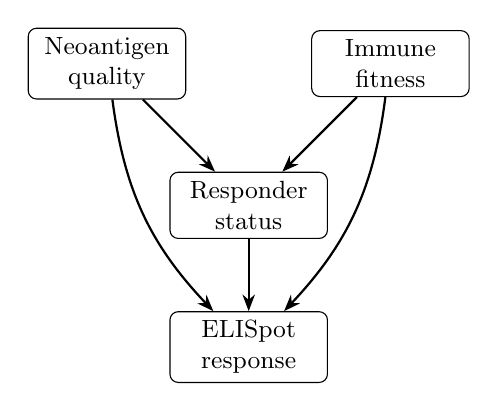
\begin{tikzpicture}[
  every node/.style={draw, rounded corners=3pt, fill=white,
                     font=\small, align=center,
                     minimum width=2.0cm, minimum height=0.65cm},
  arr/.style={-{Stealth[length=6pt]}, thick},
]
  \node (Q) at (0, 0)    {Neoantigen\\quality};
  \node (F) at (3.6, 0)  {Immune\\fitness};
  \node (R) at (1.8, -1.8) {Responder\\status};
  \node (E) at (1.8, -3.6) {ELISpot\\response};

  \draw[arr] (Q) -- (R);
  \draw[arr] (F) -- (R);
  \draw[arr] (R) -- (E);
  \draw[arr] (Q) to[bend right=18] (E);
  \draw[arr] (F) to[bend left=18]  (E);
\end{tikzpicture}
%
\hspace{2.0cm}
%
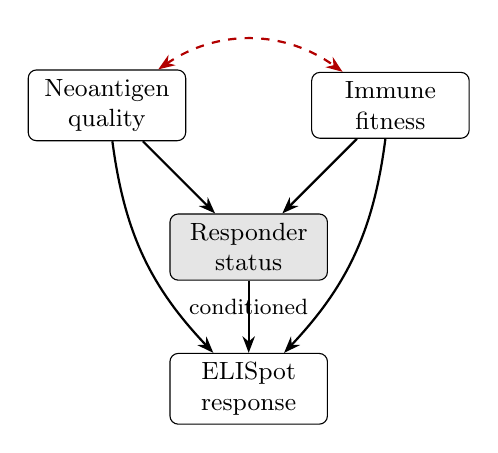
\begin{tikzpicture}[
  every node/.style={draw, rounded corners=3pt, fill=white,
                     font=\small, align=center,
                     minimum width=2.0cm, minimum height=0.65cm},
  arr/.style={-{Stealth[length=6pt]}, thick},
  spurious/.style={dashed, thick, color=red!70!black,
                   {Stealth[length=6pt]}-{Stealth[length=6pt]}},
]
  \node (Q) at (0, 0)    {Neoantigen\\quality};
  \node (F) at (3.6, 0)  {Immune\\fitness};
  \node (R) at (1.8, -1.8) [fill=gray!20,
        label={[font=\footnotesize]below:conditioned}]
                           {Responder\\status};
  \node (E) at (1.8, -3.6) {ELISpot\\response};

  \draw[arr] (Q) -- (R);
  \draw[arr] (F) -- (R);
  \draw[arr] (R) -- (E);
  \draw[arr] (Q) to[bend right=18] (E);
  \draw[arr] (F) to[bend left=18]  (E);
  \draw[spurious] (Q) to[bend left=35] (F);
\end{tikzpicture}

\caption{Collider bias induced by restricting analysis to
responders. Left: the uncontrolled DAG, in which neoantigen
quality and immune fitness are independent causes of responder
status and of ELISpot response. Right: conditioning on
responder status (shaded) opens a spurious bidirected path
between neoantigen quality and immune fitness (dashed red arc),
biasing the estimated quality--immunogenicity association
toward underestimation. The expanded cohort corresponds to the
left (uncontrolled) DAG: evaluating every long peptide, including those from
non-responders, leaves responder status unconditioned and the
quality--fitness path closed. The right panel depicts the bias induced by the
responder-restricted replication cohort.}
\label{fig:dags}
\end{figure}

In the filtered replication cohort the three biases act in different
directions. Collider bias attenuates
discrimination; mediator selection bias inflates it; lineage
confounding adds noise of indeterminate sign.
The net effect on the reported AUC of 0.68 in \citep{rojas2023personalized}
is therefore ambiguous, and any single AUC-based
discrimination figure derived from the filtered cohort should be understood
as a distorted reflection of the model's true discrimination
on the clinical candidate population.
The expanded cohort removes the two unit-selection biases: it
retains non-responders, closing the collider, and retains
filtered long peptides at the floor log-$F$ value, so mediator
selection no longer acts on the evaluated population. Lineage
confounding from the CD8$^{+}$/CD4$^{+}$ ELISpot readout remains and requires
lineage-resolved data. We therefore weight the expanded-cohort results toward
the shared substrate claim rather than the finer selection-regime contrast.

\paragraph{Original and context-revised PDAC refutations.}

The original tensor-complete expanded cohort contains
213 long-peptide endpoints, including 23 positive and 190 negative
observations. This original PDAC refutation retains every eligible patient and
uses the baseline score \(F=P\cdot N\cdot Q\cdot\Pi\). It asks whether the
composite models survive criticism in the full represented
PDAC context, treating patient immune fitness as contextual heterogeneity
outside the antigen-specific score.

A clinically important consideration is that several trial participants had
undergone splenectomy. Splenectomy may alter the capacity to mount or sustain
the measured immune response through a patient-level pathway outside
antigen-specific \(F\). Removing splenectomy-positive patients yields a
context-revised collection of 191 endpoints, including 19 positive and 172
negative observations. For that collection we will replace the baseline score
with \(F_{\mathrm{vac}}\) (Appendix~\ref{app:vaccine-conditioned-score}), which
explicitly represents vaccine-conditioned presentation and TCR expansion,
and repeat the same directed round robin.

This planned comparison contrasts the original end-to-end composite models
with versions revised for the PDAC context. Two features change together:
the revised cohort excludes splenectomy-positive patients, and the revised
score adds vaccine-conditioned presentation and TCR expansion. A difference
between the two graphs therefore describes the consequence of the combined
revision. The present comparison asks whether that revised biological account
changes the non-dominated survivor set. Assigning an observed change to one
feature would require two additional comparisons: splenectomy exclusion while
retaining the baseline score, and vaccine-conditioned scoring while retaining
the full cohort. Because the current revisions are confronted with the same
PDAC labels, this is an adaptive continuation of conjecture and criticism.
Future PDAC observations will provide new opportunities to refute the revised
survivors.

\subsection{SARS-CoV-2 spike-mutation cohort}

The third refutation setting is derived from \citet{cimenbozkus2025} (Fig.2E), which profiled T-cell
responses to spike mutations in variants of concern in a cohort of 12 healthy donors
who had received either mRNA-1273 or BNT162b2 vaccination encoding the Wuhan-1 spike
sequence. Blood was collected 14 days after the second dose (V2D14). T-cells were
expanded by stimulation with pooled 15mer overlapping peptides spanning spike mutations
found in Alpha, Beta, and Gamma variants, then re-stimulated with 24 individual 15mer
peptides --- each spanning a single mutation site in either the Wuhan-1 (WT) or variant
(MT) sequence --- and IFN-$\gamma$ production by CD4$^+$ and CD8$^+$ T-cell subsets
was measured by intracellular cytokine staining.

Each observation is a (peptide, donor) pair with a continuous \%IFN-$\gamma^+$ readout.
The setting contains two conditions: WT$\to$WT, in which T-cells expanded on the
Wuhan-1 pool are re-stimulated with individual Wuhan-1 peptides, and MT$\to$MT, in
which T-cells expanded on the variant pool are re-stimulated with individual variant
peptides. Full six-locus HLA typing is available for each donor.

The readout values are DMSO-adjusted \%IFN-$\gamma^+$ frequencies,
with donor-level background subtraction applied prior to analysis.
A (peptide, donor) observation is binarized as positive if the
background-subtracted frequency exceeds a minimum detection floor
$\epsilon > 0$:

\begin{equation}
Y_{ij} =
\begin{cases}
1 & \text{if } x_{ij} > \epsilon \\
0 & \text{otherwise}
\end{cases}
\label{eq:binarize}
\end{equation}

where $x_{ij}$ is the background-subtracted \%IFN-$\gamma^+$
frequency for peptide $i$ in donor $j$, and $\epsilon$ is a minimum
detection floor applied to remove residual technical noise near zero.
The cohort spans 23 mutation sites and 12 donors, producing at most
276 observations per condition per T-cell subset.

\paragraph{Causal structure and limitations.}

Several features of the data generating process bear on how discrimination
tests from this refutation setting should be interpreted.

All donors were previously vaccinated against Wuhan-1 spike prior to
the expansion assay. This affects both conditions. The WT$\to$WT
condition is the more directly affected: the vaccine encodes Wuhan-1
spike, so the expanded T-cell population is enriched for
vaccine-primed memory cells rather than naive T-cells primed in vitro.
The MT$\to$MT condition is similarly affected, because vaccine-primed
memory T-cells that cross-recognize variant peptides contribute to the
expansion and re-stimulation signal. Both conditions therefore measure
vaccine-conditioned recall and cross-recognition. Relative to a naive-repertoire
assay of de novo immunogenicity, this design compresses the dynamic range
between high- and low-scoring predictions.

The experimental unit is an unresolved donor--15mer response. Each mutation
site is covered by multiple overlapping 15mers at 5
amino acid offsets, and the re-stimulation uses individual 15mers
from the pool rather than a single peptide per site. A positive
readout therefore reflects recognition of at least one minimal epitope
contained within the responding 15mer, on at least one of the donor's
HLA alleles. The causal minimal epitope and restricting allele remain latent.
Minimal epitopes may be
9--12-mers, and each 15mer contains multiple overlapping frames of
each length. Model scoring therefore requires an aggregation strategy
over the set of (mer, HLA) pairs induced by the donor's six-locus HLA
type, of which taking the maximum or the mean of the top-$k$ scores
are special cases.

The readout is dominated by CD4$^+$ responses: anti-spike T-cells
are predominantly CD4$^+$ in vaccinated donors~\citep{cimenbozkus2025},
and the model targets the MHC class~I--restricted CD8$^+$ pathway.
CD8$^+$ signal is present but sparse, and point estimates of
CD8$^+$-specific discrimination will be sensitive to the small number
of positive (peptide, donor) pairs in that subset.
\subsection{SARS-CoV-2 non-spike cohort}

The fourth refutation setting is derived from \citet{cimenbozkus2025} (Fig.~4A),
which deconvolved T-cell responses to individual non-spike SARS-CoV-2
epitopes in a cohort of 13 unvaccinated convalescent patients (ATLAS
cohort). T-cells were expanded by stimulation with pooled 15mer
overlapping peptides spanning selected regions of non-spike proteins,
including the entire nucleocapsid (N) and selected regions of membrane
(M), envelope (E), ORF3a, ORF6, and ORF7a/b. Expanded T-cells were
then re-stimulated with the individual 15mer peptides constituting
those pools, and polyfunctional cytokine production
(IFN-$\gamma^+$/TNF-$\alpha^+$) by CD4$^+$ and CD8$^+$ T-cell subsets
was measured by intracellular cytokine staining. Full six-locus HLA
typing is available for each patient.

Each observation is a (peptide, patient) pair with a continuous
\%IFN-$\gamma^+$/TNF-$\alpha^+$ readout reported after donor-level
DMSO background subtraction. Per-patient binary labels are derived
by applying the same detection-floor binarization defined in
Equation~\ref{eq:binarize}, yielding a positive label if the
specific patient's background-subtracted response exceeds $\epsilon$
and a negative label otherwise. Combined with per-patient HLA typing,
this produces (peptide, patient, HLA, label) tuples directly usable
for model scoring.

\paragraph{Relationship to the spike-mutation cohort.}

This cohort complements the spike-mutation cohort in several respects.
The donors are unvaccinated convalescent patients rather than vaccine
recipients, removing the dominant Wuhan-1 spike memory priming that
compresses dynamic range in the Fig.~2E data. The peptide source is
also broader, spanning selected regions of multiple non-spike proteins
rather than 23 mutation sites within spike alone, which tests
generalization across a wider sequence and protein space. Together
these differences mean the two SARS-CoV-2 refutation settings probe the model under
distinct biological conditions while sharing the same fundamental
refutation task: binary immunogenicity classification at the
(peptide, donor) level using the binarization defined in
Equation~\ref{eq:binarize}.

\paragraph{Causal structure and limitations.}

Several features of the data generating process bear on how discrimination
tests from this refutation setting should be interpreted.

The expansion pools cover selected regions of non-spike proteins rather than
their complete sequences. Detection is therefore conditional on priming by
those selected regions. Responses to peptides outside the pools remain
unobserved, leaving the corresponding false-negative rate unidentified from
these data. Per-patient positivity should consequently be interpreted as
recognition conditional on pool-level priming.

As with the spike cohort, the experimental unit remains unresolved at the
minimal-epitope level, and CD8$^+$ responses are again sparser than CD4$^+$
responses.

% ============================================================
% RESULTS
% ============================================================

\section{Results}
\label{sec:results}

\subsection{Composite models span resolved and unresolved experimental units}

A recognition geometry and selection-decision regime, evaluated under one
component construction, give an \(\mathrm{L1}\) score for each minimal
epitope--HLA observation. Each score is the maximum of that observation's
\(F\) tensor over exposure for the specified regime and construction
(Equation~\eqref{eq:l1_score}). These scores directly confront the NCI labels.
For a long peptide, an \(\mathrm{L2}\) rule combines the candidate
minimal-epitope--HLA scores into one prediction that can confront its response
label. A complete composite model therefore specifies
\begin{equation}
M=(g,d,c,A_{\ell}),
\label{eq:composite_roster}
\end{equation}
where \(g\) is the recognition geometry, \(d\) the selection-decision regime,
\(c\) the component construction, and \(A_{\ell}\) the aggregation rule.
Varying these choices produces the full roster \(\mathcal{V}\) of competing
models, each with predictions in all four contexts.

Two models that differ only in their aggregation rule make identical NCI
predictions. The long-peptide datasets can distinguish them because they
confront the aggregated scores. Those datasets also criticize the underlying
\(\mathrm{L1}\) choices: changing the geometry, decisions, or component
construction changes the scores being aggregated. The full tournament allows
all four datasets to bear on these complete models before any alternatives
are removed through operational preference in a single context.

\subsection{Each biological context can exclude a composite model}

Suppose two models, A and B, rank the same PDAC observations differently. An
empirical advantage for A becomes a supported claim to replace B only if it
survives the declared challenges. PR/CNAP examines whether the advantage
persists across target prevalences; AUROC examines its dependence on the
weights assigned to represented positive and negative cases. Paired
computational challenges examine its dependence on combinations of the
observed units. Supported magnitude and literal survival summarize these
comparisons under the policy specified in
Appendix~\ref{app:supported-tournament}.

A supported loss in PDAC excludes B from a claim of admissibility throughout
all four contexts. B's performance elsewhere cannot cancel that loss, and A
need not also replace B in NCI or either SARS-CoV-2 cohort. Each context can
expose a deficiency, possibly through a different rival. Applying this rule to
every model pair leaves a survivor set in each context. The joint survivors
are the models common to all four sets:
\begin{equation}
S_0=S_{\mathrm{NCI}}\cap S_{\mathrm{PDAC}}
\cap S_{\mathrm{spike}}\cap S_{\mathrm{nonspike}}.
\label{eq:joint_admissibility}
\end{equation}
Here \(S_e\) contains the models with no supported incoming loss in context
\(e\) under the current policy. The graph formulation and the conditions
justifying this exclusion rule are given in
Appendix~\ref{app:supported-tournament}.

The intersection may contain several models or none. Several survivors mean
that the specified comparisons have not excluded those alternatives; an empty
set means that no model in the roster survives every context. If practical use
requires choosing among several survivors, operational rules can express a
preference without changing which models passed the criticism policy. The
survivor set \(S_0\) is therefore retained separately from the operational
selection. PR/CNAP and AUROC produce separate sets over the same model roster;
neither assigns a probability to performance in an unrealized cohort.

\subsection{Computational limits of the full tournament}

Crossing 4,200 geometry--decision regimes with five component constructions and
seven \(\mathrm{L2}\) rules produces 147,000 composite models. Comparing every
pair in all four contexts would require approximately
\(4.32\times10^{10}\) pair--context matches per metric, with both directions
assessed in each match. Deciding which models survive need not require all of
these comparisons.

Once a model has a supported loss, further losses are unnecessary to establish
its exclusion. Establishing survival is more demanding: every rival that could
supply an incoming loss must still be accounted for. The accelerated
implementation uses this asymmetry. It rules out directions that cannot pass
the observed-metric gate and stops assessing a target within a context once a
supported loss has been found. It retains the evidence for that exclusion.
For a reported survivor, every possible incoming loss must have been assessed
or ruled out by the observed-metric gate. An assessed comparison may remain
scientifically unresolved; such a comparison supplies no supported loss.
Excluded models remain available as rivals in comparisons with other models.

This procedure preserves the joint survivor set, but its cost depends on how
many comparisons are needed to establish losses and survival. Worst-case work
remains quadratic in the number of models. If many models survive, a subsequent
operational selection can also be expensive: the current refinement requires
complete numerical comparisons among those survivors across contexts. These
costs motivate restricting the roster before constructing and comparing all
long-peptide models.

\subsection{NCI survivors define reduced composite-model rosters}

NCI can supply the first comparison because its observations require only
\(\mathrm{L1}\) scores. Within each component construction, the NCI tournament
compares the candidate geometry--decision regimes and retains every regime
without a supported incoming loss. This survivor set is recorded before the
later operational rules select one or more preferred regimes.

Each surviving regime can then be paired with all seven \(\mathrm{L2}\)
rules. For example, a surviving full-HLA regime produces seven complete
models with the same underlying minimal-epitope scores but different rules for
combining those scores into a long-peptide prediction. Repeating this
construction for every NCI survivor across the five component constructions
produces a reduced roster for comparison in NCI, PDAC, spike, and non-spike.
Appendix~\ref{app:nci-selection} gives its formal definition.

NCI remains part of this second tournament because the initial tournaments
compare regimes only within each component construction. The second tournament
also compares models from different constructions and can therefore expose NCI
losses that the initial comparisons did not examine. The long-peptide contexts
additionally distinguish the aggregation rules and the consequences of the
underlying \(\mathrm{L1}\) scores.

This sequence preserves every regime that survived its initial NCI tournament.
Whether the resulting roster is tractable depends on how many regimes survive.
A smaller roster could be formed from the NCI operational selections or from
representatives of distinct surviving regimes, but those restrictions would
omit alternatives that NCI had not excluded through a supported loss.

\subsection{Omitted models can still supply decisive criticism}

A model can lose its eligibility to be selected while remaining useful for
criticizing another model. Suppose model A has a supported loss in NCI, but
supports replacement of model B in PDAC. The full tournament excludes A
because of its NCI loss and B because of its PDAC loss. A reduced tournament
that removes A before the PDAC comparisons may leave B's deficiency unexposed.

A model retained for its ability to supply such a comparison is a challenger,
even if it is no longer eligible to be selected. Preserving these challenger
roles separates exact staged execution from the NCI survivor approximation.
An NCI loss excludes every aggregation variant of the losing regime because
those variants share the same NCI predictions. The variants can cease to be
eligible winners, but they must remain available to challenge other models
where required by the full comparison. If the second tournament instead
compares only models constructed from NCI survivors, it can miss losses
supplied by excluded challengers.

Passing only NCI operational selections introduces another omission. A regime
that survived supported criticism but lost the NCI operational comparison might
survive the full joint tournament or become its preferred choice after another
context excludes the NCI-preferred alternative. Choosing representatives of
surviving regimes can omit such alternatives as well. Even identical NCI
rankings do not establish that two regimes make identical predictions in the
long-peptide contexts.

These omissions can be examined by expanding the restricted comparison.
Restoring excluded models as challengers tests whether they supply additional
supported losses. Restoring omitted survivors as eligible candidates tests
whether they remain admissible or change the operational selection. With the
scoring rules, observations, and criticism policy held fixed, each change can
be attributed to the added comparisons. Agreement between restricted rosters
still leaves the unexamined comparisons open. The choice of approximation
therefore depends on the number and diversity of the NCI survivors and on which
omitted comparisons can subsequently be restored.

\newpage
\begin{thebibliography}{99}

\bibitem[Mora \& Walczak(2023)]{MoraWalczak2023}
T.~Mora and A.~M. Walczak,
``Towards a quantitative theory of tolerance,''
\emph{Trends in Immunology} \textbf{44}, 512--523 (2023).
\doi{10.1016/j.it.2023.04.008}

\bibitem[Mayer et~al.(2022)]{mayer2022different}
A.~Mayer, C.~J.~Russo, Q.~Marcou, W.~Bialek, and B.~D.~Greenbaum,
``How different are self and nonself?''
\emph{arXiv preprint} arXiv:2212.12049 (2022).

\bibitem[Rojas et al.(2023)]{rojas2023personalized}
Rojas, L. A., Sethna, Z., Soares, K. C., Olcese, C., Pang, N.,
Patterson, E., Lihm, J., Ceglia, N., Guasp, P., Chu, A., et al.
Personalized RNA neoantigen vaccines stimulate T-cells in pancreatic cancer.
\textit{Nature}, 618(7963), 144--150, 2023.

\bibitem[Bozkus et~al.(2025)]{cimenbozkus2025}
Bozkus, C.C., Brown, M., Velazquez, L., Thomas, M., Wilson, E.A., O'Donnell, T.,
Kaminska, A., Ruchnewitz, D., Geertz, D., Bykov, Y., et~al.
\newblock T-cell epitope mapping reveals immunodominance of evolutionarily
conserved regions within {SARS-CoV-2} proteome.
\newblock {\em iScience}, 28(8), 2025.
\end{thebibliography}

\newpage
\appendix

\section{NCI screening and operational selection}
\label{app:nci-selection}

For each component construction, the NCI roster contains 4,200
geometry--decision regimes. Every observation is scored by the same maximum
over its six exposure values within each regime. The complete roster includes
steepness variants and regimes with identical score vectors; empirical AP and
AUROC do not screen their inclusion. Separate PR/CNAP and AUROC tournaments
apply the supported-replacement policy to these scores.

The fixed-policy graph reduction produces \(S_{0,\mathrm{NCI},c}\), the
surviving geometry--decision regimes for component construction \(c\).
Let \(\mathcal{C}\) contain the five component constructions and
\(\mathcal{A}\) the seven aggregation rules. The full composite-model roster is
\(\mathcal{V}=\mathcal{G}\times\mathcal{D}\times\mathcal{C}\times\mathcal{A}\).
Expanding every component-specific NCI survivor into all aggregation variants
gives
\begin{equation}
\mathcal{V}_{\mathrm{NCI}}
=\bigcup_{c\in\mathcal{C}}
\left\{(g,d,c,A_{\ell}):
(g,d)\in S_{0,\mathrm{NCI},c},\ A_{\ell}\in\mathcal{A}\right\}.
\label{eq:nci_expansion}
\end{equation}
These initial survivor sets are metric-specific. They omit cross-component
NCI comparisons and can therefore retain regimes that a pooled NCI tournament
would exclude.

When an operational selection is requested, every member of
\(S_{0,\mathrm{NCI},c}\) remains an eligible candidate and challenger. For each candidate, incoming activation
strengths are sorted from greatest to least. Their vectors are minimized
lexicographically, comparing the strongest threat first and proceeding to the
next coordinate only on a tie. The resulting set \(T\) may remain plural.

Only then is metric-specific regret compared, retaining all of
\(S_{0,\mathrm{NCI},c}\) as benchmarks. PR uses worst-target CNAP regret over
the declared prevalence interval. AUROC uses empirical AUROC regret at uniform
within-class weights. Identical final vectors remain tied in \(S_{\mathrm{op}}\).
For the current single-context NCI AUROC policy, empirical AUROC maximizers
survive the observed gate and have zero incoming activation profiles; the
regret rule therefore retains those maximizers. This property does not extend
to a joint comparison in which another context can exclude them.

Expanding \(S_{0,\mathrm{NCI},c}\) or expanding \(S_{\mathrm{op}}\) defines
different reduced composite-model rosters. The former preserves every regime
that passed the fixed NCI criticism policy, whereas the latter also restricts
eligibility through the NCI operational rule. Neither restricted roster alone
preserves the full joint tournament's challenger obligations.

\section{Long-peptide aggregation systems}
\label{app:l2-systems}

\paragraph{Scope and common inputs.}
A long-peptide assay supplies one label without identifying which candidate
short-peptide--HLA pair explains the response. Level~2 must map these
candidate-level predictions to one score for that experimental unit. We
specify seven alternative aggregation functions: maximum, top-two mean,
top-fraction mean, median, log-sum-exp, log-mean-exp, and a hybrid aggregation
rule. The first six directly summarize the candidate scores. The seventh
also uses peptide and allele identities, combining distinct-peptide breadth
with support through a second HLA allele; this combination is what we call
the hybrid. The functions are competing choices for \(\mathrm{L2}\), not
successive stages of the calculation. This appendix defines the common inputs
and the six direct summaries before developing the hybrid.

For a fixed geometry--decision regime and component construction, let
\(S_{jh}\geq0\) be the candidate \(\mathrm{L1}\) score and write
\(z_{jh}=\log(S_{jh}+\epsilon)\), with \(\epsilon=10^{-12}\).
Here \(j\) indexes a distinct short-peptide sequence and \(h\) its
candidate restricting allele. Each peptide--HLA tuple is counted once, giving
\(K\) candidate pairs. All seven functions receive this same indexed
collection of log scores.

All seven rules are endpoint-local: they use only the endpoint's candidate
scores and identities and constants fixed before scoring. Adding an unrelated
long peptide to a batch therefore cannot change an existing endpoint's score.
Each rule is applied unchanged across the five component constructions and
all geometry--decision regimes; it leaves the underlying \(\mathrm{L1}\)
component calculations unchanged.

\paragraph{Six direct score summaries.}
For these operators, flatten the candidate roster to \(z_1,\ldots,z_K\)
and order the values as \(z_{(1)}\geq\cdots\geq z_{(K)}\). Define
\(k_2=\min(2,K)\) and \(k_f=\max(1,\lceil0.02K\rceil)\) for a
nonempty roster. The definitions and the information retained by each
summary are:

\begin{center}
\small
\begin{tabular}{@{}p{0.22\linewidth}p{0.32\linewidth}p{0.37\linewidth}@{}}
\toprule
Function & Definition & Information retained \\
\midrule
Maximum & \(z_{(1)}\)
& The strongest candidate alone \\
\addlinespace
Top-two mean & \(k_2^{-1}\sum_{i=1}^{k_2}z_{(i)}\)
& The mean of the leading two log scores \\
\addlinespace
Top-fraction mean & \(k_f^{-1}\sum_{i=1}^{k_f}z_{(i)}\)
& The mean of the leading 2\% of log scores \\
\addlinespace
Median & \(\operatorname{median}(z_1,\ldots,z_K)\)
& The center of the log-score distribution \\
\addlinespace
Log-sum-exp & \(\log\!\left(\sum_{i=1}^{K}e^{z_i}\right)\)
& Accumulated positive-scale signal over all pairs \\
\addlinespace
Log-mean-exp & \(\log\!\left(K^{-1}\sum_{i=1}^{K}e^{z_i}\right)\)
& Positive-scale accumulation normalized by pair count \\
\bottomrule
\end{tabular}
\end{center}

The two upper-tail means average log scores; log-mean-exp averages their
exponentials before taking the logarithm. These are different operations.
All six functions depend only on the multiset of scores: reassigning those
scores among peptide and allele identities leaves their outputs unchanged.
Consequently, they do not distinguish whether additional high scores belong
to different peptides or to one peptide paired with several alleles.

\paragraph{Why add a hybrid alternative?}
Maximum protects a strong candidate from dilution by numerous weak
alternatives, but discards all secondary support. The other direct summaries
retain additional scores without distinguishing their peptide and allele
identities. The hybrid combines a maximum anchor with two separate summaries
of additional support. It makes three commitments: preserve the strongest
candidate's score, allow additional candidate support to raise it, and
distinguish support across peptide sequences from support through different
HLA alleles. These are modeling hypotheses, not properties uniquely
determined by the assay. The six direct summaries remain alternatives against
which those choices can be assessed.

\begin{minipage}{\linewidth}
\paragraph{Two summaries of the peptide-by-HLA matrix.}
For the hybrid, view the same roster as a matrix whose rows are distinct
short-peptide sequences \(j\) and whose columns are distinct candidate
restricting alleles \(h\). Retaining the maximum along each row or column
answers a different question:
\[
\underbrace{u_j=\max_h z_{jh}}_{\text{best score for peptide }j},
\qquad
\underbrace{b_h=\max_j z_{jh}}_{\text{best score for allele }h}.
\]
\end{minipage}\par\smallskip
Both summaries retain the same overall maximum,
\(m=\max_j u_j=\max_h b_h\), but discard different information. The
following configurations illustrate the distinction; ``strong'' describes
candidate model scores, not experimentally confirmed epitopes or calibrated
response probabilities.

\begin{center}
\small
\begin{tabular}{@{}p{0.37\linewidth}p{0.27\linewidth}p{0.27\linewidth}@{}}
\toprule
Candidate-score pattern & Peptide-level support & HLA-level support \\
\midrule
One strong peptide--HLA pair
& One leading peptide & One leading allele \\
\addlinespace
Several strong peptides,\newline one allele
& Additional peptides & One leading allele \\
\addlinespace
One strong peptide,\newline several alleles
& One leading peptide & Additional alleles \\
\addlinespace
Several strong peptides,\newline several alleles
& Additional peptides & Additional alleles \\
\bottomrule
\end{tabular}
\end{center}

Row maxima give each peptide one contribution, preventing its scores under
several alleles from being counted as several distinct peptides. Column
maxima recover information about alternative alleles that row maxima may
discard. Neither distinct sequences nor distinct alleles imply independent
biological evidence: candidate peptides can overlap, and the two summaries
come from the same roster.

\paragraph{The score as a maximum plus two increments.}
Let \(\Delta_{\mathrm{pep}}\) denote the admitted peptide-support increment
and \(\Delta_{\mathrm{HLA}}\) the bounded second-allele increment, defined
below. The final score is
\begin{equation}
S_{\mathrm{hybrid}}
=m+(1-w)\Delta_{\mathrm{pep}}+w\Delta_{\mathrm{HLA}},
\qquad 0\leq w\leq1.
\label{eq:l2_hybrid}
\end{equation}
This form separates the protected maximum from the two forms of
corroboration. With \(s_{\mathrm{pep}}=m+\Delta_{\mathrm{pep}}\) and
\(s_{\mathrm{HLA}}=m+\Delta_{\mathrm{HLA}}\), it is equivalently the convex
combination \((1-w)s_{\mathrm{pep}}+w s_{\mathrm{HLA}}\).
Convex weighting is an additional modeling choice that controls the tradeoff
between the increments. Increasing \(w\) raises the coefficient of HLA
support and lowers that of peptide support; it does not append an HLA bonus
to an unchanged peptide score. Retaining the shared maximum once does not by
itself require this particular weighting.

\paragraph{The available peptide-support increment.}
On the row-collapsed roster, let \(x_j=\max_h S_{jh}\) be each peptide's
positive-scale signal before addition of the numerical floor. For a nonzero
roster, define
\[
T=\sum_j x_j,\qquad M=\max_j x_j,\qquad
R=\frac{T}{M},\qquad p_j=\frac{x_j}{T}.
\]
The ratio \(R\) measures total signal relative to the strongest peptide.
It equals one if only one peptide carries positive signal, and equals \(n\)
if exactly \(n\) peptides carry equal positive signal. More generally it is
the order-infinity Hill effective number,
\(N_\infty=1/\max_j p_j=R\), rather than a literal count of peptides.

The collapsed log-sum score \(U=\log(T+\epsilon)\) exceeds the maximum
\(m=\log(M+\epsilon)\) by an available accumulation \(U-m\).
Temper this accumulation by the fraction of signal outside the leader:
\begin{align*}
D&=1-\max_j p_j=1-\frac1R,\\
C_{\mathrm{pep}}&=D\max(U-m,0)
=\left(1-\frac1R\right)
\log\!\left(\frac{T+\epsilon}{M+\epsilon}\right).
\end{align*}
The maximum with zero is a numerical safeguard, since \(T\geq M\).
When \(M\) is large relative to the numerical floor,
\[
C_{\mathrm{pep}}\approx\left(1-\frac1R\right)\log R.
\]
Thus the two factors depend on the same effective-breadth ratio; they are
not independently varying descriptions of the roster. Their product
suppresses small amounts of nonleading signal more strongly than the
untempered accumulation: if \(R=1+r\) with small positive \(r\), then,
away from the floor, \(C_{\mathrm{pep}}\approx r^2\), whereas
\(U-m\approx r\).

This summary has a specific limitation. Rosters with the same maximum and
total receive the same offer regardless of how their remaining signal is
divided. For example, positive-scale rosters \((1,1)\) and
\((1,\tfrac12,\tfrac12)\) have the same \(M\), \(T\), and
\(C_{\mathrm{pep}}\), despite containing different numbers of nonzero
peptides. The offer captures dominance-based effective breadth after
sequence collapse, not the full distribution of peptide support.

\paragraph{Admitting peptide support through a self-limiting gate.}
The available offer does not specify how much should influence the final
score. We conjecture that peptide corroboration should contribute less as
the resulting score becomes strong. A decreasing sigmoid implements this
choice smoothly; the assay does not require either that conjecture or this
particular functional form. Write the admitted increment as
\begin{equation}
\Delta_{\mathrm{pep}}
=C_{\mathrm{pep}}\,
\sigma\!\left(\frac{c_{\mathrm{pep}}-m-\Delta_{\mathrm{pep}}}
{\kappa_{\mathrm{pep}}}\right),
\qquad \sigma(v)=\frac{1}{1+e^{-v}},
\label{eq:l2_peptide_gate}
\end{equation}
with \(s_{\mathrm{pep}}=m+\Delta_{\mathrm{pep}}\) and
\(\kappa_{\mathrm{pep}}>0\). The center \(c_{\mathrm{pep}}\) is the
resulting score at which half the offer is admitted; the width
\(\kappa_{\mathrm{pep}}\) controls the smoothness of that transition.

The offer raises the score, while that rise reduces the fraction admitted.
This negative feedback explains why the increment appears on both sides of
Equation~\ref{eq:l2_peptide_gate}. Gating only on \(m\) would fix the
fraction before the increase occurred. Here the left side increases with
\(\Delta_{\mathrm{pep}}\) and the right side is nonincreasing; their
intersection exists uniquely in \([0,C_{\mathrm{pep}}]\).

The sharp-transition limit makes the behavior explicit. Holding all other
quantities fixed gives
\[
s_{\mathrm{pep}}\xrightarrow{\kappa_{\mathrm{pep}}\to0^+}
m+\min\!\left\{C_{\mathrm{pep}},(c_{\mathrm{pep}}-m)_+\right\},
\qquad (a)_+=\max(a,0).
\]
In this limit, a maximum below the center receives the full offer if the
resulting score would remain below the center; otherwise it rises only to
the center. A maximum already above the center is preserved. For positive
transition width the behavior is smooth, and the center is not a strict cap.

\paragraph{Qualifying support through a second HLA allele.}
The allele maxima \(b_h\) retain information about additional alleles even
when the same short peptide supplies their strongest scores. Let
\(b_{(2)}\) be the second-largest maximum among distinct alleles. Its
own strength qualifies the additional route: a small gap from the leader
would also reward two similarly weak scores. An increasing sigmoid admits
a fraction of a nonnegative bonus cap \(B\):
\begin{equation}
\Delta_{\mathrm{HLA}}
=B\sigma\!\left(\frac{b_{(2)}-t_{\mathrm{HLA}}}
{\delta_{\mathrm{HLA}}}\right),
\qquad s_{\mathrm{HLA}}=m+\Delta_{\mathrm{HLA}},
\label{eq:l2_hla_gate}
\end{equation}
where \(\delta_{\mathrm{HLA}}>0\). The bonus is \(B/2\) when
\(b_{(2)}=t_{\mathrm{HLA}}\), and the positive width controls the
transition. The second allele's strongest candidate may be the same peptide
as the leading allele's candidate or a different one.

The gates answer different questions. The decreasing peptide gate regulates
how much an available accumulation may raise the resulting score; the
increasing HLA gate assesses whether a second allele's input score warrants
a bonus. Adding that bonus does not change \(b_{(2)}\), so the HLA gate
requires no self-consistency equation. Both sigmoids are deterministic
scoring operations, not response probabilities or established biological
thresholds.

\paragraph{Bounds, limiting cases, and score scale.}
The increments satisfy \(0\leq\Delta_{\mathrm{pep}}\leq C_{\mathrm{pep}}\)
and \(0\leq\Delta_{\mathrm{HLA}}\leq B\). Consequently,
\[
m\leq S_{\mathrm{hybrid}}
\leq m+(1-w)C_{\mathrm{pep}}+wB.
\]
Neither branch dilutes the strongest candidate, and the HLA contribution
cannot exceed \(wB\). A single positive peptide gives no peptide offer,
but can still receive HLA corroboration if it has support through a second
allele. Conversely, a roster with several supported peptides but only one
represented allele can supply peptide breadth without an HLA increment.
With \(w=0\), the score
is the peptide branch; with \(w=1\), it is the HLA branch.

Relative breadth and absolute score location play different roles. Multiplying
every positive-scale candidate score by a common positive factor leaves
\(R\) unchanged. Away from the numerical floor it also leaves
\(C_{\mathrm{pep}}\) unchanged, but shifts the log scores entering the
gates. The gate centers therefore refer to the specified \(\mathrm{L1}\)
score scale. With fixed centers, the admitted increments can change under
rescaling even when relative breadth does not.

\paragraph{Numerical conventions.}
The numerical floor is \(\epsilon=10^{-12}\). In computation, recover the
positive-scale peptide signal from its log score by
\(x_j=\max(e^{u_j}-\epsilon,0)\) before forming \(T\), \(M\), and
\(p_j\). Otherwise the floor would itself accumulate as apparent support.
An empty roster, or a roster with every \(x_j=0\), returns
\(\log\epsilon\) before normalization. When fewer than two distinct
alleles are represented, set \(\Delta_{\mathrm{HLA}}=0\).
Bisection solves the peptide equation within
\([m,m+C_{\mathrm{pep}}]\) for \(s_{\mathrm{pep}}\), to an absolute
bracket width of \(10^{-10}\), with at most 64 iterations.

\paragraph{Calibration of the hybrid.}
The functional form leaves the gate locations, widths, bonus cap, and mixture
weight unspecified. Calibration used completed full-HLA candidate scores in PDAC, COVID spike, and
COVID nonspike. Candidate structures and parameterizations were compared with
the same full-HLA fixed-maximum reference within each context. The staged
paired-CNAP assessment used 600 computational replications and required a
positive supported magnitude with survival above zero exceeding 0.81 in every
context. Eligibility was therefore conjunctive across contexts. The comparisons
informed successive structural and numerical revisions, rather than selecting
the final hybrid from a single grid declared before development.

The frozen specification is
\[
(c_{\mathrm{pep}},\kappa_{\mathrm{pep}},t_{\mathrm{HLA}},
\delta_{\mathrm{HLA}},B,w)
=(-2.2,0.13,-6.45,0.02,1,0.12).
\]
It admits half the peptide offer at \(s_{\mathrm{pep}}=-2.2\) and half
the HLA bonus at \(b_{(2)}=-6.45\). The mixture assigns weights 0.88 and
0.12 to the peptide and HLA branches, respectively, limiting the final HLA
increment to 0.12 log-score units.
A local sensitivity assessment held the peptide gate fixed and evaluated the
Cartesian product
\begin{align*}
t_{\mathrm{HLA}}&\in\{-6.475,-6.45,-6.425\},
&\delta_{\mathrm{HLA}}&\in\{0.015,0.020,0.025\},\\
B&\in\{0.50,0.75,1.00\},
&w&\in\{0.08,0.10,0.12\}.
\end{align*}
Each of these 81 parameterizations was assessed by the same paired criterion
in all three contexts to probe sensitivity to the numerical choices.
The frozen specification above is used unchanged for
both tournament metrics and every component construction. Response labels
informed its development, but neither labels nor context identity enter its
endpoint-scoring function.

The seven aggregation rules and five component constructions define 35
composite models for each geometry--decision regime. Crossing these models
with 4,200 regimes gives the 147,000-model roster used for both metrics. Each
NCI survivor contributes seven aggregation variants to a reduced roster.

\section{Supported-superiority tournament policy}
\label{app:supported-tournament}

Each pair of composite models supplies two directed replacement claims within
each of the four contexts. The proposed comparison retains the NCI policy:
supported magnitude must exceed zero, and literal survival above zero must
exceed 0.81 under order-two computational challenges formed from 600 paired
replications. PR uses prior-standardized average precision over target
prevalences from 1\% to 30\%, expressed as
\(\mathrm{CNAP}_{\pi}=(\mathrm{AP}_{\pi}-\pi)/(1-\pi)\).
AUROC challenges the paired advantage by varying within-class case weights.
The observed anchor and computational assessment must both meet the declared
requirements; neither metric uses an exchangeable-label reference law.

Every context supplies a separate assessment. The comparison preserves model
pairing on the same experimental units, and its computational construction must
specify which units are resampled together to preserve the dependencies admitted
by that context. Repeated observations and linked patient or peptide records
require an explicit unit specification. Neither pooling all cohort rows nor
averaging cohort advantages implements the candidate-conservative rule.

A context's supported directions form a graph \(G_e\), with an edge from
the supported replacement to the model it exceeds. A strongly connected
component contains models joined by directed paths in both directions. A
source component has no incoming edge from another component. The models in
these source components form the context's maximal set,
\(S_e=\operatorname{srcSCC}(G_e)\). Candidate-conservative selection intersects
these sets:
\[
S_0=\bigcap_{e\in\mathcal{E}}\operatorname{srcSCC}(G_e),
\qquad
\mathcal{E}=\{\mathrm{NCI},\mathrm{PDAC},\mathrm{spike},\mathrm{nonspike}\}.
\]
The strict observed CNAP and AUROC gates provide increasing scalar potentials
for supported directions under the current policy, so each context graph is
acyclic. Its source components are individual models with no incoming
supported loss, as used in Equation~\eqref{eq:joint_admissibility}. One incoming
edge therefore supplies an exclusion witness.

The alternative replacement-conservative policy first intersects the directed
edge sets and then finds the source components of the resulting graph. It
requires the same replacement direction to be supported in every context.
Different rivals can therefore expose a model's deficiencies in different
contexts without excluding it from this alternative selection. The
candidate-conservative rule instead allows each context to exclude a model
through its own supported comparisons.

Accelerated candidate-conservative execution certifies exclusions and resolves
survivor obligations against the full declared roster. An excluded model
remains a challenger. Reuse of identical scores or paired computations must
preserve the scientific policy, computational design, seeds, and audit
bindings; shared predictions alone do not authorize substituting an existing
match artifact. The accelerated output certifies selection and need not contain
a complete graph or the alternative replacement-conservative reduction.

Operational refinement freezes the joint \(S_0\) as both candidate and
challenger set. Incoming vectors combine activation strengths across contexts
and challengers and are minimized lexicographically. If several candidates
remain in \(T\), PR compares worst-target CNAP regrets against every member of
\(S_0\); AUROC compares empirical AUROC regrets in each context. Descending
context-regret vectors are minimized lexicographically, and exact ties remain
ties. Complete numerical reports among survivors are required for this
refinement even when fewer reports suffice to certify \(S_0\).

A sequential approximation must record its stage-specific candidate and
challenger sets. Removing a model from eligibility after a supported NCI loss
can preserve the joint selection; removing its unassessed challenger roles can
omit exclusions elsewhere. A restriction based on operational preference or
representative selection can additionally omit eligible candidates. Changing
those restrictions, the spike observation definition, or the PDAC scoring and
inclusion rules defines a revised comparison whose conclusions must retain
that provenance.


\section{Vaccine-conditioned extension of the immunogenicity score}
\label{app:vaccine-conditioned-score}

In a vaccine setting, the immune system is exposed to a
coordinated set of vaccine-derived peptides at high effective concentration. This
creates an additional layer of structure. Vaccine-derived n-mers compete with one
another for presentation, and the resulting pMHC complexes can expand the TCR
clones available to recognize related peptide--HLA contexts.

Let \(\mathcal V\) denote the set of vaccine-derived n-mers induced by the
administered long peptides. For each \(e\in\mathcal V\), we define a vaccine-context
binding bid
\[
b_{\mathrm{vac}}(e,h)
=
\frac{[P_e]_{\mathrm{vac}}\,S(e,h)}{K_d(e,h)},
\qquad
\widetilde b_{\mathrm{vac}}(e,h)
=
[M_{h,\mathrm{tot}}]\,b_{\mathrm{vac}}(e,h),
\]
where \([P_e]_{\mathrm{vac}}\) is the effective vaccine-derived peptide supply.
The corresponding vaccine presentation measure is
\[
Q_{\mathrm{vac}}(e,h,\mathcal{H},\mathcal{V})
=
\frac{\widetilde b_{\mathrm{vac}}(e,h)}
{
\sum_{h'\in \mathcal{H}}[M_{h',\mathrm{ref}}]
+
\sum_{h'\in \mathcal{H}}
\left(
C^{\mathrm{ref}}_{h',\mathrm{self}}(\gamma)
+
\sum_{e'\in\mathcal V}
\widetilde b_{\mathrm{vac}}(e',h')
\right)
}.
\]
This expression uses the same calibrated-background normalization as \(Q\), with
the query set replaced by the full vaccine-derived peptide set. High vaccine
supply increases the total vaccine bid mass, which is then divided
competitively among vaccine-derived n-mers. Each n-mer receives a share of the
available HLA-specific presentation capacity according to the strength of its
binding bid relative to endogenous background and to the bids of the other
vaccine-derived n-mers. Relative presentation therefore remains selective even
under strong vaccine loading.

We next define the vaccine-induced stimulation load for a scored observation
\(o=(e,h,\mathcal{H})\):
\[
A_{\mathrm{vac}}(o)
=
\sum_{v\in\mathcal V}
K_{\mathrm{TCR}}(o,v)\,
Q_{\mathrm{vac}}(v).
\]
Here \(K_{\mathrm{TCR}}(o,v)\) encodes sharing of TCR recognition between the scored
observation \(o\) and the vaccine-derived pMHC \(v\). The simplest choice is an
identity kernel, where only the same n-mer--HLA pair contributes. More general
kernels can assign partial weight to related pMHCs that are expected to share
cross-reactive TCR clones.

We convert this stimulation load into a bounded expansion term,
\[
E_{\mathrm{vac}}(o)
=
\beta
\frac{A_{\mathrm{vac}}(o)^\alpha}
     {K_A^\alpha + A_{\mathrm{vac}}(o)^\alpha},
\]
where \(\beta\) is the maximal additive vaccine-induced expansion term, so that
the largest possible multiplicative increase in effective TCR availability is
\(1+\beta\). \(K_A\) is the stimulation level at which expansion reaches half
of its maximal value, and \(\alpha\) controls the sharpness of the transition.

The vaccine-conditioned score scales effective TCR availability
\(P\cdot N\) by \(1+E_{\mathrm{vac}}\):
\begin{equation}
F_{\mathrm{vac}}(e,h,\mathcal{H},\mathcal{S};\theta)
=
P(e,\mathcal{H},\mathcal{S};\theta)
\cdot
N(e,\mathcal{H},\mathcal{S};\theta)
\cdot
Q(e,h,\mathcal{H},\mathcal{S})
\cdot
\left(1+E_{\mathrm{vac}}(e,h,\mathcal{H},\mathcal{V})\right)
\cdot
\Pi(e,h).
\label{eq:F_vac_corrected}
\end{equation}

In the initial implementation, we use the identity form of \(K_{\mathrm{TCR}}\) and
treat \(\beta\), \(K_A\), and \(\alpha\) as global calibration parameters. The
values used in a vaccine-conditioned tournament specify the vaccine-conditioned
terms of the revised composite models and are recorded before their pairwise
comparisons are formed. Extensions with
cross-reactive kernels or exhaustion terms can be introduced once the data
support those additional degrees of freedom.

\paragraph{Scale of the vaccine expansion parameters.}

The parameters in \(E_{\mathrm{vac}}\) should be interpreted on the scale of the
stimulation load \(A_{\mathrm{vac}}\), not on the scale of administered vaccine
dose. In the identity-kernel implementation, \(A_{\mathrm{vac}}(e,h)\) is simply
the vaccine-context presentation share \(Q_{\mathrm{vac}}(e,h,\mathcal{H},\mathcal{V})\) for the same
peptide--HLA pair. Thus, \(K_A\) represents the per-observation vaccine
presentation level required for half-maximal expansion. A value such as
\(K_A=1\) would place half-maximal expansion at the extreme where essentially
all vaccine-context presentation mass is concentrated in a single
peptide--HLA observation. Competition among many vaccine-derived n-mers places
the empirical \(A_{\mathrm{vac}}\) distribution well below that scale. We
therefore set or fit \(K_A\) relative to the empirical distribution of
\(A_{\mathrm{vac}}\) values.
For example, choosing \(K_A\) near the upper tail of this distribution makes
expansion selective for the most strongly presented vaccine pMHCs, whereas a
smaller \(K_A\) allows moderate presentation levels to induce appreciable
expansion. The parameter \(\beta\) controls the maximal possible additive
increase in effective TCR availability, while \(\alpha\) controls how sharply
expansion transitions around \(K_A\).

In the default implementation, we use \(\rho_{\mathrm{vac}}=2\),
\(\beta=1\), \(K_A=10^{-2}\), and \(\alpha=1\). The choice
\(\rho_{\mathrm{vac}}=2\) sets the total vaccine-derived bid mass to twice the
calibrated endogenous self-background bid mass, representing a strong but not
dominant vaccine presentation pressure. The choice \(\beta=1\) allows vaccine
exposure to at most double the effective TCR availability term through the
factor \(1+E_{\mathrm{vac}}\). The value \(K_A=10^{-2}\) means that a
peptide--HLA observation reaching approximately one percent vaccine-context
presentation share attains half-maximal expansion. Finally, \(\alpha=1\) gives a
smooth Michaelis--Menten-like transition rather than an abrupt threshold. These
defaults serve as interpretable starting values whose biological adequacy is
examined through calibration and sensitivity analysis.

\paragraph{Status of the vaccine-conditioned score.}

The baseline score \(F=P\cdot N\cdot Q\cdot\Pi\) and the vaccine-conditioned
score \(F_{\mathrm{vac}}\) define different PDAC predictions. A comparison must
specify which version supplies the PDAC context and fix its vaccine parameters
before assessing the resulting composite models. Replacing the baseline
predictions with vaccine-conditioned predictions is a revision of that
context's scoring rule. Combining this change with splenectomy exclusion also
changes the admitted observations, so attribution requires the separate
comparisons described in the PDAC refutation data. These revisions continue
conjecture and criticism against the existing PDAC evidence.

\paragraph{Bid-level parameterization of vaccine peptide supply}

Administered RNA or peptide dose provides only indirect information about the
intracellular supply of individual vaccine-derived n-mers. Processing,
expression, and degradation intervene between administered dose and the
peptides available for HLA loading. In parallel, the endogenous background term
\(C^{\mathrm{ref}}_{h,\mathrm{self}}(\gamma)\) is a calibrated effective
competition scale. We therefore parameterize vaccine supply at the level most
relevant to the presentation model: the relative bid mass of vaccine-derived
peptides compared with the endogenous self background.

Let
\[
B_{\mathrm{self}}(\mathcal{H},\gamma)
=
\sum_{h\in \mathcal{H}} C^{\mathrm{ref}}_{h,\mathrm{self}}(\gamma)
\]
denote the total calibrated self-background bid scale for HLA environment \(\mathcal{H}\)
and context class \(\gamma\). We introduce a dimensionless implementation
parameter \(\rho_{\mathrm{vac}}\), defined so that the total vaccine-derived bid
mass satisfies
\[
\sum_{h\in \mathcal{H}}\sum_{e\in\mathcal V}
\widetilde b_{\mathrm{vac}}(e,h)
=
\rho_{\mathrm{vac}}\,
B_{\mathrm{self}}(\mathcal{H},\gamma).
\]
Thus, \(\rho_{\mathrm{vac}}=1\) corresponds to vaccine-derived competitive
pressure comparable to the calibrated endogenous self background, while larger
or smaller values represent stronger or weaker vaccine loading, respectively.

To convert \(\rho_{\mathrm{vac}}\) into peptide-level supplies, we assign each
vaccine-derived n-mer a nonnegative relative supply weight \(u_e\). In the
simplest implementation, \(u_e=1\) for all \(e\in\mathcal V\). We then set
\[
[P_e]_{\mathrm{vac}} = c_{\mathrm{vac}} u_e,
\]
where the scale factor \(c_{\mathrm{vac}}\) is chosen to enforce the desired
total vaccine bid mass:
\[
c_{\mathrm{vac}}
=
\frac{
\rho_{\mathrm{vac}} B_{\mathrm{self}}(\mathcal{H},\gamma)
}{
\sum_{h\in \mathcal{H}}\sum_{e\in\mathcal V}
[M_{h,\mathrm{tot}}]\,
u_e\,S(e,h)/K_d(e,h)
}.
\]
This yields
\[
\widetilde b_{\mathrm{vac}}(e,h)
=
[M_{h,\mathrm{tot}}]\,
\frac{c_{\mathrm{vac}}u_e S(e,h)}{K_d(e,h)}.
\]

Under this parameterization, \([P_e]_{\mathrm{vac}}\) is an effective coordinate
on a relative presentation-competition scale. The resulting bid preserves the
model's dependence on peptide--HLA binding strength, stability, HLA environment,
and the endogenous calibrated background.





\end{document}
